\documentclass[a4]{report}
\usepackage[english]{babel}
\usepackage[utf8]{inputenc}
\usepackage{graphicx}
\usepackage{fancyhdr}
\usepackage[export]{adjustbox}

\pagestyle{fancy}
\fancyhf{}
\lhead{Uppsala University}
\cfoot{\thepage}
\rfoot{Mohammadmahdi Amini}
\renewcommand{\headrulewidth}{0.5pt}
\renewcommand{\footrulewidth}{0.5pt}

\begin{document}

    \begin{titlepage}

        \begin{figure}
            \begin{minipage}{0.48\textwidth}
                \begin{flushleft}
                    
\includegraphics[scale=0.5]{images/UU_LOGO.png}
                \end{flushleft}
            \end{minipage}\hfill
            \begin{minipage}{0.48\textwidth}
                \begin{flushright}
                    
\includegraphics[scale=0.5]{images/UU_LOGO.png}
                \end{flushright}
            \end{minipage}
        \end{figure}

        \thispagestyle{fancy}

        \vspace{1in}

        \center

        \textsc{\large MASTER THESIS REPORT}

        \vspace{0.5in}

        \noindent\makebox[\linewidth]{\rule{\linewidth}{1.2pt}}
        \textsc{ \textbf{\large FenceX: High throughput scalable geofencing }}
        \noindent\makebox[\linewidth]{\rule{\linewidth}{1.2pt}}

        \vspace{0.5in}

        \begin{minipage}{0.48\textwidth}
            \begin{flushleft}
                \textit{Student:} \\
                Mohammadmahdi Amini \\
                mm7amini@gmail.com
            \end{flushleft}
        \end{minipage}
        \begin{minipage}{0.48\textwidth}
            \begin{flushright}
                \textit{Supervisor:} \\
                Salman Toor \\
                salman.toor@it.uu.se
            \end{flushright}
        \end{minipage}

        \vspace{2in}

        \textbf{\large Department of Information Technologies} \\

        \today

    \end{titlepage}

    \null\newpage
    \setcounter{page}{2}

    \section{abstract}
    Since emergence of smartphones, smart cars and other mobile objects with GPS sensor attached to them, (non-)
    functional requirement of geofencing systems has significantly changed.
    Previously, the number of mobile objects thus the size of geospatial data about them and their load on the
    geofencing systems were much lower.
    Also, geofencing services were not much integrated in the day to day life of nonprofessional users.
    Nowadays, on the other hand, geofencing systems are required to process large loads of requests and data in
    realtime with a very high availability for much wider range of users.
    FenceX is a geofencing system that supports both realtime and on demand geofencing in a highly scalable manner.
    FenceX delivers geofencing with high throughput and is designed with resiliency and availability in mind.
    The main pillars of FenceX are stream processing and microservices which resulted in a reactive distributed
    system.
    FenceX has shown weak and strong scalability characteristics while being evaluated using real taxi trip data.
    Apart from being a geofencing system, FenceX can be considered an implementation for the idea of stateful function
    as a service.
    This has been achieved by allowing custom implementation for stream processing operations in the pipeline.
    Since FenceX has both stateful and stateless operations, it can be considered a stateful FAAS platform.
    While comparing FenceX with other works done, we observed better results in multiple dimensions, peak throughput
    and resiliency for example.

    \newpage

    \tableofcontents

    \listoffigures

    \listoftables

    \newpage

    \section{Acknowledgment}
    Huge thanks and appreciations to all people who had a hand in the actualization of FenceX.
    First and foremost, my supervisor, Salman Toor, who trusted in me and my idea.
    Without his continues feedback and support FenceX wouldn't make it to existence.
    Also reviewer of this thesis, Sadi Alawadi, whose feedback was necessary to keep the work relevant and scientific.
    Special appreciation to Snic cloud who provided us with computational resources needed for evaluation of FenceX
    under project 2020/20-3.
    Also, Cabonline and my manager there at time,  Emil Ekdahl, for providing us with real taxi trip data
    (anonymized) which we have used intensively in the evaluation phase.
    Last but not least my friend and ex-college, Juan Fandino, whose work was inspirational for FenceX.

    \section{Open source}
    All of the work has been done during this thesis including reports and implementations is available in
    a Github repository (github.com/bmd007/statefull-geofencing-faas).
    The content of this repository is available to be used openly.
    Please feel free to contribute as well.

    \chapter{Introduction}
    ?

    \chapter{Related work}
    ?

    \chapter{Geofencing}
    Geofencing essentially is checking whether a geospatial point is inside a geospatial shape or not.
    This can be done in two styles: push and poll.
    In poll style, a fence (geospatial shape) is queried against a database of coordinates (mover-id:geospatial point).
    The result is all coordinates residing in the fence.
    This type of geofencing relies on geospatial indexing.
    So updating and querying the database of coordinates is CPU intensive.

    On the other hand in push style, fences are pretty much predefined.
    Whenever coordinates of a mover changes (a location update report arrives), an intersection check between a
    predefined fence and the newly reported coordinate will happen.
    Although no geospatial indexing is necessarily involved, the intersection checking operation is still CPU
    intensive due to the required mathematical calculations.

    We can compare these two styles as following:
    \begin{itemize}
        \item In poll style we have a \textbf{database of locations} and in push style, a \textbf{database of fences}.
        \item Poll style geofencing has an \textbf{on demand} nature while push style is of \textbf{real time} nature.
        \item Poll style fencing use case examples: Taxi/police/ambulance dispatch, disaster management.
        \item Push style fencing use case examples: Elderly/Kid/Pet care, (gambling) addiction management.
    \end{itemize}

    Please note that using poll/push terminology is an idea brought up in this thesis in order to facilitate
    conversations about different approaches to geofencing.

    \paragraph{}
    In order to represent geospatial data several standards (formats) are available, namely WKT\cite{WKT}, WKB\cite{wkb},
    GeoJSON\cite{geoJson} and GML\cite{gml}.
    Please check the data presentation standard upon which they are based in the table \ref{table:geofencing-formats}.

    \begin{table}[h!]
        \centering
        \begin{tabular}{|c|c|}
            \hline
            Geofencing format & Parent data format \\
            \hline
            GeoJSON           & JSON               \\
            GML               & XML                \\
            WKB               & Binary             \\
            WKT               & Plain text         \\
            \hline
        \end{tabular}
        \caption{Base standard of Geofencing formats}
        \label{table:geofencing-formats}
    \end{table}

    We can compare the geofencing representations mentioned in the table \ref{table:geofencing-formats} fundamentally
    in the same way in which we compare their corresponding base standards.

    In this thesis we used WKT to represent all the involved geospatial data.
    We have chosen WKT since our geospatial database (index) of choice, H2, supports it well.
    Also, we couldn't find any information about H2 supporting other geospatial representations out of the box.

    \subsection{WKT}
    WKT (well known text) is a text mark up language which is a format for geometric information.
    Items below are examples of WKT strings representing raw geometry data.
    \begin{itemize}
        \item POINT(6 10): a point with x=6 and y=10
        \item LINESTRING(3 4,10 50,20 25): a line consisting of 3 points.
        \item POLYGON((1 1,5 1,5 5,1 5,1 1),(2 2, 3 2, 3 3, 2 3,2 2)): two squres one convering the other
        \item MULTIPOINT((3.5 5.6),(4.8 10.5)): just two points
        \item MULTILINESTRING((3 4,10 50,20 25),(-5 -8,-10 -8,-15 -4)): two lines
        \item MULTIPOLYGON(((1 1,5 1,5 5,1 5,1 1),(2 2, 3 2, 3 3, 2 3,2 2)),((3 3,6 2,6 4,3 3)))
        \item GEOMETRYCOLLECTION(POINT(4 6),LINESTRING(4 6,7 10))
        \item POINT ZM (1 1 5 60)
        \item POINT M (1 1 80)
        \item POINT EMPTY
        \item MULTIPOLYGON EMPTY
    \end{itemize}

    Instead of relative values for X,Y and Z, geographic coordinates (latitude, longitude) can be used in order to
    represent geospatial data.
    We mainly used POINT() to model locations and MULTIPOLYGON() for fences.

    \begin{figure}[ht]
        \centering
        \caption{Texas WKT illustration}
        \label{fig:texas}
        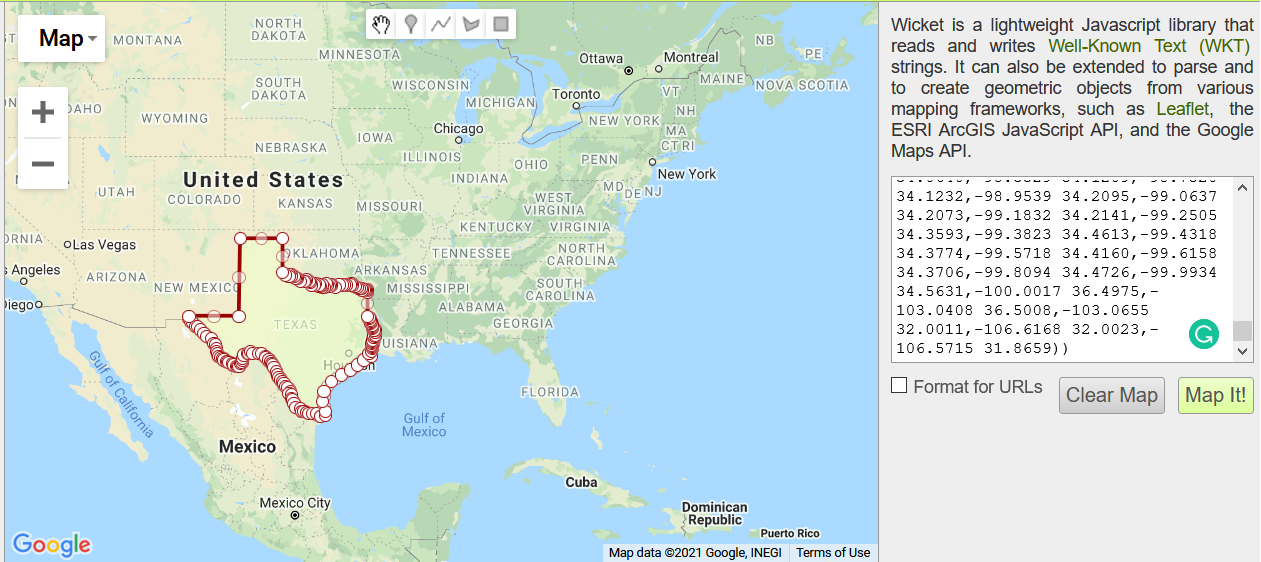
\includegraphics[width=\linewidth, scale=0.5]{images/texas.png}
    \end{figure}
    Figure \ref{fig:texas} illustrates usage of an online tool \cite{WKTtool} to show a geospatial WKT on a map.
    The WKT refers to borders of state Texas in US which is taken from \cite{WKTs}.

    \section{Requirements}
    Both styles of geofencing are CPU intensive.
    Also, geofencing is usually implemented using databases interacting with disk and accessed over network.
    So a combination of natural computational latency and IO latency limits the overall throughput of geofencing systems.
    This gets worst in high load high scale use cases.
    Which means the higher the load, the higher the effect of aforementioned latencies on the overall performance
    of the system.
    As a remedy we can improve the computational aspect of the problem by improving the indexing algorithms.
    However, usually the IO latency is much more effective than operational burden.
    So the other approach to improve the throughput is using co-located in memory databases which do not interact
    with disk and are accessed through local network (localhost).
    In this thesis we focused on the later and tried to minimize the IO latency.

    \paragraph{}
    We decided to use co-located in memory databases to minimize IO.
    Everything will be fine until our systems faces an amount of load which can not be handled properly even after scaling up.
    At this stage we scale the system out and deploy more than one instance of the program.
    This will also help with resiliency of system;
    if one of the instances of program goes down or stops responding for some reason, the system can still keep
    serving with remaining available instances.

    \paragraph{}
    Until now, we achieved high throughput, scalability and resiliency by minimizing IO latency and scaling the
    application out.
    Which means we ended up with a distributed system containing some components (instances of our application) that
    need to have same image of world, same data more precisely.
    The location updates or queries sent to the system by clients, can end up in any of the available instances due
    to load balancing.
    Otherwise, there should be way to shard the data between instances and tell clients how to select the correct
    instance to which send a location update or query.
    We went for replication over sharding with hope of keeping clients and data management simple.
    So we need to somehow make those instances have the same image of the world (same data) otherwise, their results
    will be inconsistent.

    So far we have exchanged IO for the holly inconsistency issue of distributed systems.
    So the challenge is to keep the throughput, scalability and resiliency of geofencing system high while avoiding
    inconsistency among it's components.

    \subsection{Functional requirements}
    Movers want their location reports be received by FenceX.
    This report contains the coordinate (latitude, longitude) at which mover was located when producing the report.
    A timestamp might be included in the report as well.

    Movers want their latest reported location to be available for being queried by their ID (Movers want their
    latest reported location be memorised by system).

    Users want to be able to send a geospatial shape (fence) to the system and in turn get movers (id:location) who
    are in the fence (according to their latest location report) = on demand fencing

    Users want to be able to create/update/remove/query a fence (geospatial shape) for each mover (by id).

    Movers expect each of the location reports to be checked against a potential fence.
    Which mean for each location report for each mover, potentially a fence-point intersection should be calculated.
    The result of each intersection is if the reported coordinate located within the predefined fence.
    In case no fence is defined for a specific mover, no fence-point intersection should be calculated.

    \subsection{Non-functional requirements}
    As a result of required system being a general geofencing provider, the required precision of system might vary
    based on the users and use cases.
    So FenceX should be able to ingest very high rates of location reports.
    Looking at potential use cases, in some the report rate could be like one report per mover every 1 minute and
    maximum of 1K active movers at the same time.
    Other cases might involve 1 location report per mover every 5 second with 1M active movers.
    So FenceX should have a very high capacity to handle load and stress.

    Since based on the use case, the required scalability of system may differ, the users of system should be able to
    tune the system according to their needs.
    Or at least the fact that scalability requirements are not fixed over time should be factored in the design,

    Availability of FenceX should relay on modules so that if something goes wrong in one part of it, the other parts
    keep working.
    If FenceX stops receiving location reports, for instance, it should be still possible to query the saved
    locations by mover id and/or fence.
    In some cases it is acceptable to miss some location updates for some movers while in others, missing location
    reports is not tolerable due to high precision requirements.

    The time that takes for FenceX to answer a query by fence or calculate a fence-point intersection should not be a
    factor of the incoming load.
    In other words, the latency of those two operations should be reasonably low and should not increase as the load
    on the system increases.
    Such low latency will play a important role in the overall throughput of FenceX.

    Consistency level required for geofencing applications is not strong so eventual consistency will suffice.
    Once a location report has received, it might takes a fraction of time until the view of FenceX about
    corresponding mover changes.
    Before that, latest previously captured report and finalized view is valid and used.
    Same goes for predefined fences.
    So no need for distributed transactions or implementation of Saga as there is not much of intertwined
    interactions that can go wrong.

    \chapter{FenceX}
    FenceX is a stream processing system designed and implemented into microservices.
    It can also be identified as a reactive distributed system that is applying event driven architecture for
    communication of its modules.
    These four big software architectural names are pretty much the same thing in the context of FenceX with their
    point of view being different.
    To avoid repeating same vocabulary over and over in this document, we use the terminology specific to each of
    these realms interchangeably more precisely when applicable.
    The listing below illustrates words that refer to similar things but originate from different terminologies.

    \begin{itemize}
        \item  \textbf{Microservice:} microservice, service, operation, event processor, processor, subscriber,
        publisher, module and subsystem.
        \item \textbf{Instance:} instance, task.
    \end{itemize}

    \section{System overview}
    As you can see in the figure \ref{fig:logical-dfg}, FenceX has 6 operators.
    Some of them are stateful and backed by a state store and some of them are stateless.
    The exact details are as below in relation to state:

    \begin{itemize}
        \item \textbf{Stateful:} location-aggregate, fence-aggregate, location-fence-intersection
        \item \textbf{Stateless:} location-update-publisher (source), filter
    \end{itemize}

    \begin{figure}[ht]
        \centering
        \caption{Logical data flow graph of FenceX}
        \label{fig:logical-dfg}
        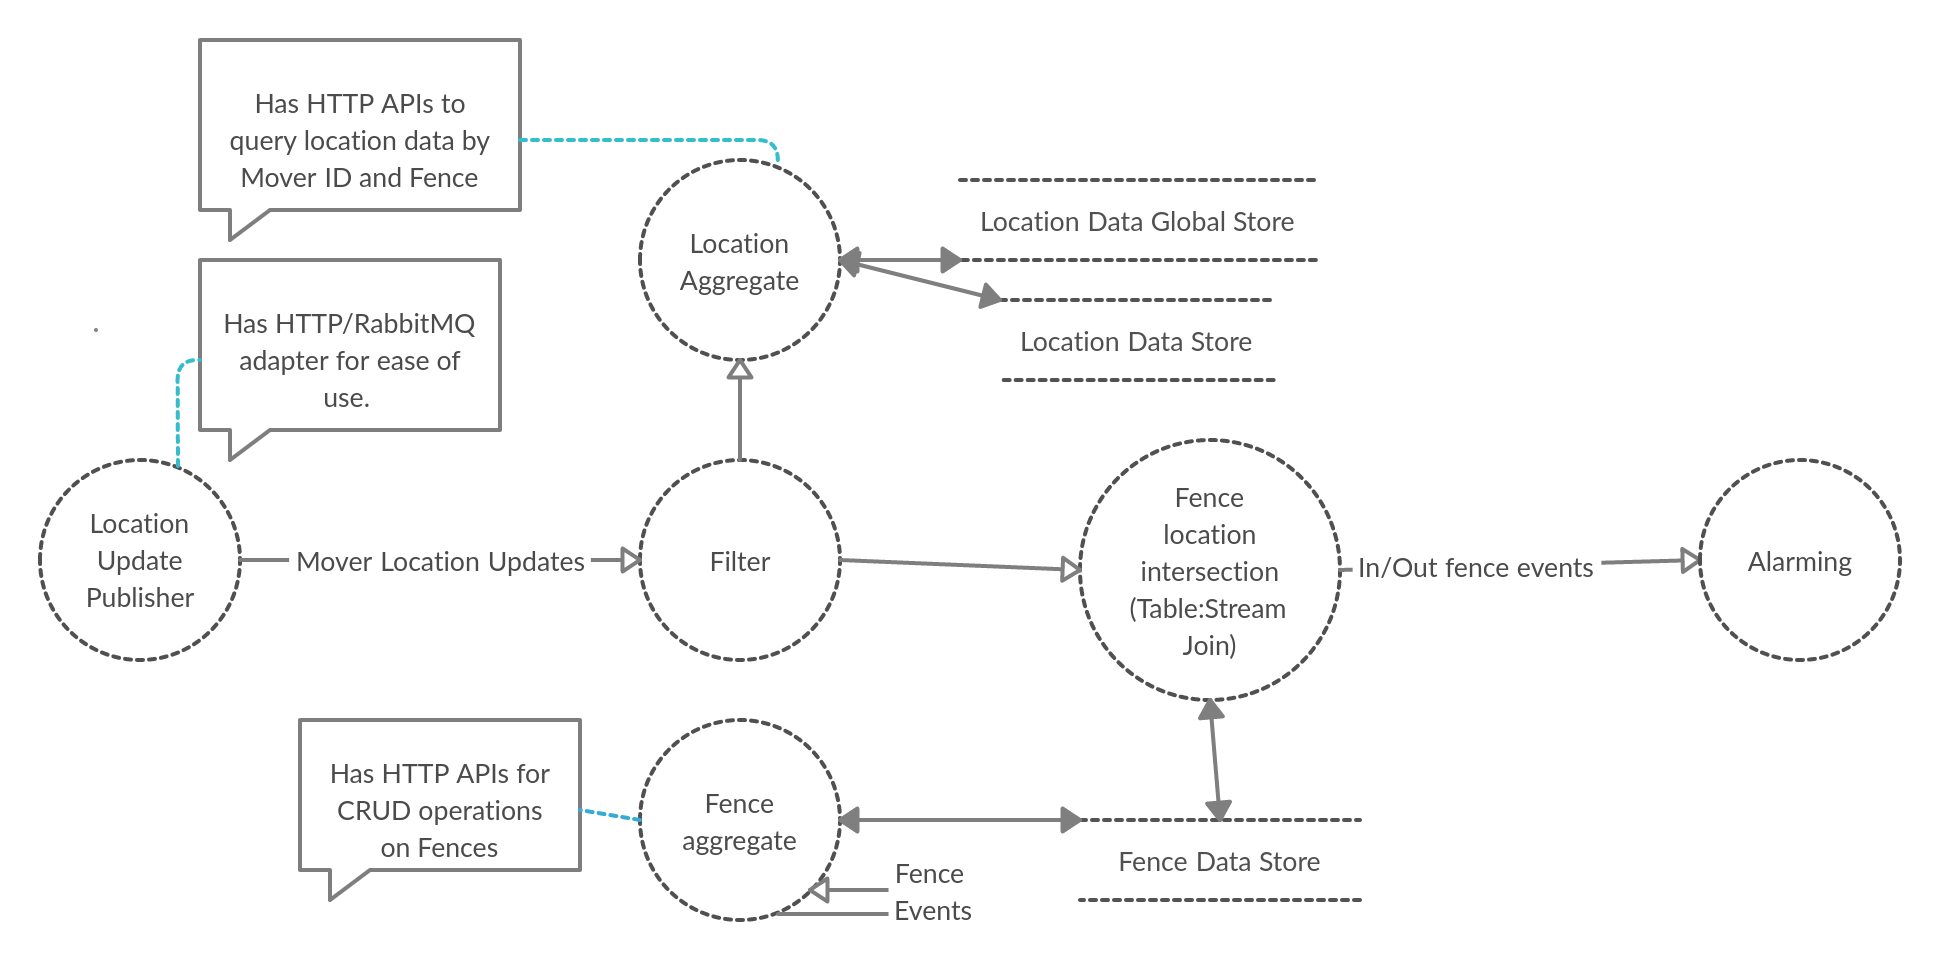
\includegraphics[width=\linewidth ,scale=0.2]{images/logical-data-flow-diagram.png}
    \end{figure}

    \paragraph{location-update-publisher} plays the role of source in the FenceX stream processing pipeline.
    It has HTTP and RabbitMQ adaptors which is used by movers.
    Movers send messages or HTTP requests in order report their latest location.
    Location-update-publisher turns each report into an event and publishes it into a kafka topic called
    \textbf{location-updates}.

    \paragraph{filter}, as the name suggests, is responsible for avoiding not desired location updates to find their
    way further down the stream.
    Checks can be against null values or invalid latitude/longitude.

    \paragraph{location-aggregate} is responsible for keeping a view of the latest location of each mover by
    subscribing to the stream of location updates coming out of filter.
    It has a local database of mover-locations which applies geospatial index on the data.
    As a result, the query by fence becomes possible.
    So location-aggregate is responsible for answering queries both by mover id and fence (geospatial shape).

    \paragraph{fence-aggregate} is responsible to keep track of predefined fences (for real time intersection scenarios).
    It exposes HTTP APIs for CRUD operations.
    The fences are kept in a temporal KTable (kafka streams notion of table) and backed by a durable Kafka topic.
    In other words, each operation (CRUD) on each fence is initially a Kafka event which is later processed by
    fence-aggregate into a fence.
    The producer of those events is also fence-aggregate.
    In more technical terms, fence-aggregate is using event-sourcing architecture internally.

    \paragraph{fence-location-intersection} (join) has a view of predefined fences (managed by fence-aggregate) in
    shape of a key:value table.
    Key is id of mover for which the fence (value) is defined.
    fence-location-intersection is a join between that table and stream of location updates coming out of filter.
    Those location updates also has a key:value form.
    Key is the mover id and value is the reported location.
    And finally, the join operation is to check if the fence in table contains the location in the update.
    The result of this intersection will be events like mover X is (not) in the predefined fence.

    \paragraph{alarming} is responsible for responding to the events coming out of fence-location-intersection.
    Implementation of this operator is not withing boundaries of this thesis.
    So we won't describe it in details.

    \subsection{Push and Poll legs}
    As described previously, FenceX provides two styles of geofencing, on demand and real time.

    Sending HTTP queries with a geospatial fence (query by fence) to FenceX is of on demand nature.
    Which means when ever a client demands a geofencing operation, they send a HTTP query.
    In this style, fences are very dynamic.
    The fence will be checked against the whole database of mover locations.
    \textbf{location-aggregate} is responsible for this style of fencing.
    Since sending query to a system is like polling data out of it, the parts of FenceX making this possible are
    considered poll leg.
    So \textbf{location-aggregate} is poll leg of FenceX.

    Calculating fence-point intersection for every location report, on the other hand, is of real time nature.
    For each new location report, system pushes a intersection calculation result.
    \textbf{fence-location-intersection and fence-aggregate} carry the burden of real time fencing and they are the
    push leg of FenceX.
    In this style the defined fences are more static and don't change frequently over time.

    From now on, we will use the notions of push and poll leg frequently specially in the evaluation phase, Each of
    these legs have their own characteristics and require individual attention.

    \section{Physical data flow graph}
    \begin{figure}[ht]
        \centering
        \caption{Physical data flow graph of FenceX}
        \label{fig:physical-dfg}
        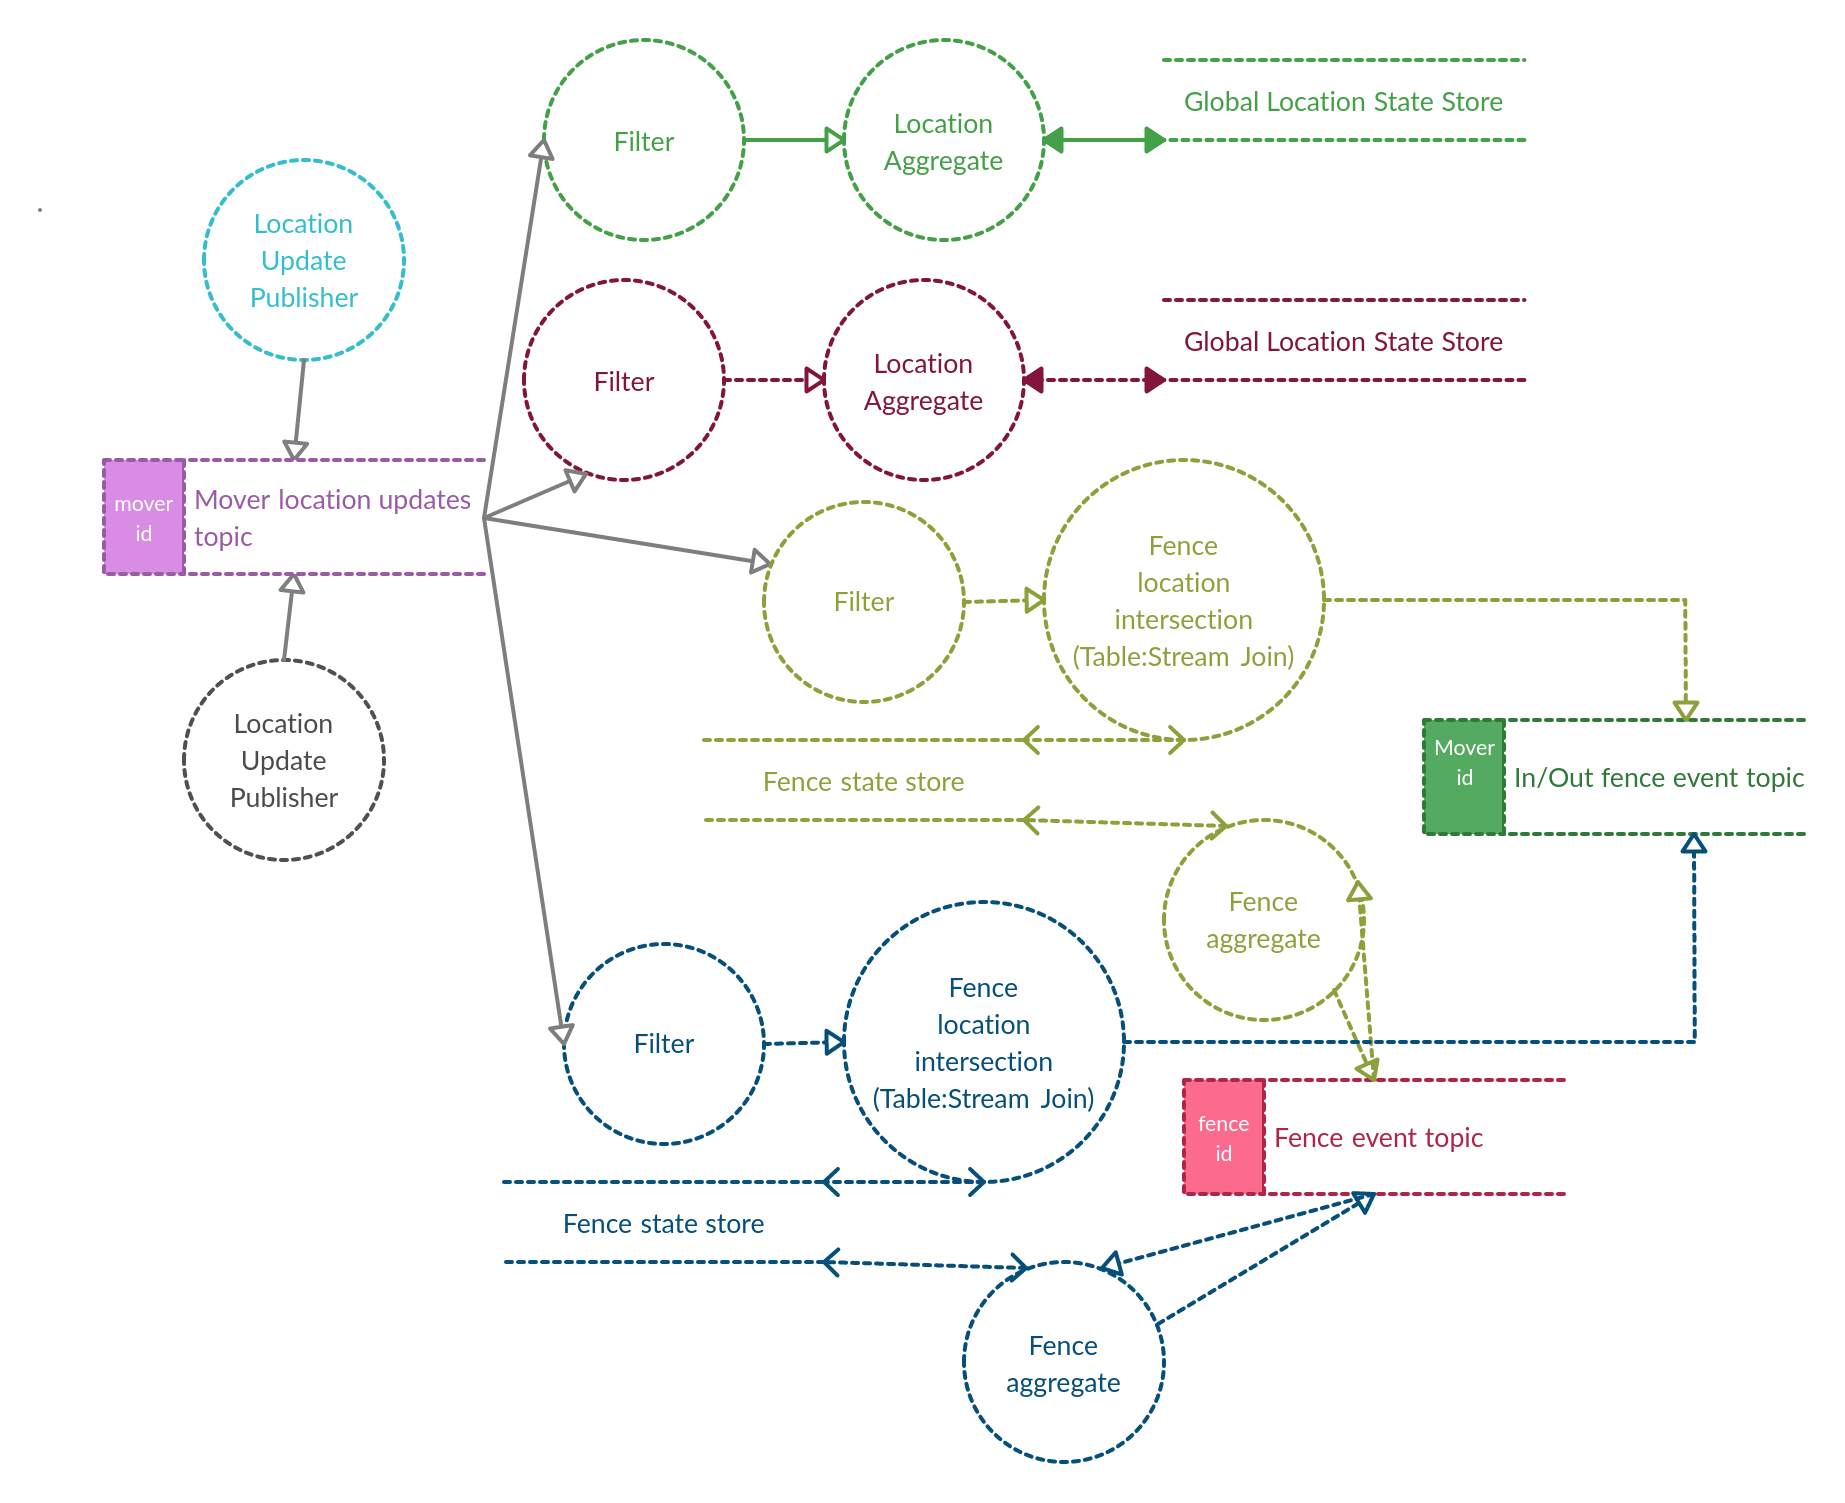
\includegraphics[width=\linewidth ,scale=0.2]{images/physical-data-flow-diagram.png}
    \end{figure}

    Figure \ref{fig:physical-dfg} is a physical data flow graph, illustrating how possibly FenceX components can be
    deployed as instances of microservices containing stream processing pipeline tasks.
    Each group of tasks that has similar color, are one unit of deployment, an instance of a microservice.

    The combination of tasks below will be deployed as one microservice:
    \begin{itemize}
        \item{location-update-publisher} alone makes a microservice called \textbf{location-update-publisher}.
        \item{filter and location-aggregate} together make a microservice called \textbf{location-aggregate}. This the poll leg of FenceX.
        \item{filter, fence-aggregate and fence-location-intersection} together make a microservice called \textbf{realtime-fencing}. This the push leg of FenceX.
    \end{itemize}

    You can see that each microservice exists two times in \ref{fig:physical-dfg} differed by color.
    It means FenseX deploys more than one instance of each microservice for scalability and resiliency purposes.
    Such characteristics will be discussed in details later.

    Below are the facts common about all FenceX microservices:
    \begin{itemize}
        \item They are implemented using Java 15.
        \item They are implemented with extensive help from Spring family frameworks and libraries like Spring boot, Spring data, Spring webflux, Spring cloud and many more.
        \item They are packaged as layered docker images, so the deployment artifacts of FenceX are docker images.
        \item So far all of them expose some HTTP APIs implemented using Spring webflux on top of project reactor.
        As a result they are reactive applications which means they process HTTP requests in an asynchronous and non blocking manner.
        \item All of them expose a HTTP API for fetching metrics about their resource usage, JVM status, geofencing
        operations and some other metrics.
        \item After successful deployment, they will be registered into a service discovery tool called Consul\cite{Consul}.
    \end{itemize}

    \subsection{Inter microservices communication}
    At the moment there is no need for HTTP communication between FenceX microservices.
    However, they can find each other's IP by querying Consul on the fly.

    The communication style of microservices in FenceX is asynchronous and event driven.
    Which means there are Kakfa topics available for publishing events and subscribing to them.
    This topics are partitioned so each instance of the microservice will subscribe to a sub set of partitions.
    This is a load sharing strategy which helps with scalability.
    Figure \ref{fig:physical-dfg} illustrates involved (Kafka) topics in the pipeline in addition to the state
    stores(database) attached to/used by each task.
    Fundamentally each of those state stores are backed by a topic (changelog).


    \section{Microservices internal design and implentation}
    Apart from common fact stated preciously, FenceX microservices can be described in a more detailed way as following:

    \subsection{location-update-publisher}
    Location-update-publisher is a simple Kafka publisher.
    A source in the stream processing pipeline.
    It can be exposed to outside world using both RabbitMQ and HTTP adapters.
    The adapters receive location reports.
    Reports will be mapped to the event schema that other microservices
    understand and finally the event will be published into a topic called \textbf{location-updates}.
    This is a stateless service, so it can be scaled out very easy.
    Since the functionality of this service is simple, each instance doesn't need to be rich in resources.

    \subsection{location-aggregate}
    Location-aggregate is a Kafka Streams application.
    It's internal stream starts with subscribing to \textbf{location-updates}, continues with a filter and finally
    aggregated into a Global KTable which is backed by an in-memory H2 database.
    Which means once a location report received by location-aggregate, it will be first checked for validity and then
    saved into an in-memory co-located database.
    The save is an update operation most of the time.
    Updating the latest captured location for a mover.
    H2 provides geospatial indexing.
    Upon each update, the index will be updated as well, so that the database will become ready for queries (query by
    fence).
    By database though, we mean a single big table here.

    \subsubsection{Co-located database}
    Usually in information systems, databases have their own cluster and deployed on machines other than the one on
    which applications are deployed.
    This is done in order to abstract away availability and scalability challenges of data(base) from developers.
    The disadvantage is that accessing such a database can only happen over network which is an IO operation with
    relatively high latency.
    Since we aimed for high throughput (low latency) geofencing in FenceX, we decided to use a databases process
    deployed tightly together with location-aggregate.
    The life cycle of this database is managed by location-aggregate.
    In fact, it's a library within the application.
    In summary, we used an embedded database.
    The direct result is that the network call for accessing this database is only within range of localhost, so the
    latency is minimum.

    \subsubsection{In memory database}
    Usually database systems are configured to use disk as storage which allows them to grow very big.
    The downside with this approach is the IO intensiveness of interacting with disk which means latency.
    Although very high throughput SSD hard drives exists, not only their price tag is high but also they are still
    not as fast as memory.
    Our goal being minimizing IO latency, the H2 database not only is configured to use memory as storage but also
    using it in an asynchronous non-blocking manner (nioMemFS).
    Which means H2 will act as if a file system exists on the memory and will access it using Java NIO \cite{JavaNio} technology.

    \subsubsection{Inconsistency}
    Using database systems maintaining their own dedicated cluster, means no need for being worry about the
    possible inconsistency problems.
    The nodes in the cluster need to be consistent after all, even if only they act as cold idle replicas.
    Co-located in memory databases, on the other hand, usually doesn't have any consideration for replication and/or
    consistency.
    Since we want to scale out poll leg of FenceX, facing inconsistency issues is inevitable.
    So we need a way to make each instances of location-aggregate (all of the H2 instances) have same data, same
    image of the world.
    H2 provides an out-of-the-box solution for keeping its instances consistent, even when configured to be embedded
    and in memory.
    However, after some trial and error we did not find it reliable.
    So it is up to us to keep the instances of location-aggregate consistent.
    Kafka Streams Global KTables are state stores that have same data regardless of instance.
    They are equivalent to kafka subscribers each having a different group name;
    which means they get events from all partitions.
    Normal KTables only keep a subset of world image which corresponds to the partitions they listen to.

    So if we put the H2 database underneath a Global KTable, Kafka Streams out of box keeps the H2 instances
    consistent.
    \textbf{Eventually consistent} However!
    Eventually consistent means the consistency of data among instances of location-aggregate is not of ACID nature.
    Once a location update is published, the time taking for each instance to capture the location update and change
    its state accordingly, varies from an instance to another.
    This time is a factor of, for example, current load of each instance.

    Each Kafka Streams state store is backed by a topic called change log.
    This topic is durable and is saved on disk by kafka.
    Each Kafka Streams application attached on such a store, subscribe to that topic once it's up and running and
    populate its KTables.
    That topic contains all changes that has happened to the state of application, the data in the KTable.
    So in case something happens to one of the instances (or all of them for that matter), after a restart or bringing
    a new fresh instance up, the instance recover/creates it own images of the world just by subscribing to change
    log topic.
    The subscription can be from last seen offset or from offset zero, depending on the state of underlying store.
    Sometimes the stores are backed by a database using file system as storage.

    So finally we resolved the mystery of inconsistency in FenceX. Also, we covered some aspects of the work which
    makes FenceX high throughput.

    \subsection{realtime-fencing}
    Realtime-fencing is a Kafka Streams application responsible for keeping track of fences, receiving location updates
    and joining them.
    The join operation is fence-point intersection.
    It has two internal streams.
    One for processing location updates, and the other is for aggregating fences.

    \subsubsection{Event-sourcing}
    One of the internal streams starts with subscribing to \textbf{fence\_event\_log} topic.
    The publisher to this topic is realtime-fencing itself.
    It exposes two HTTP APIs for CRUD operations on fences (only create is implemented for now).
    For instance, when create fence API is called, apart from possible initial validations, the
    only thing that happens is that an (kafka) event will be published to the \textbf{fence\_event\_log} topic.
    \textbf{fenceCreatedEvent} in this case.
    No fence is created yet or saved anywhere in the system, however that's how an event-sourcing based application
    works.
    The stream that starts with subscribing to \textbf{fence\_event\_log} topic, receives those events and aggregates
    them into a Kafka Streams KTable.
    A key:value table in which key is the ID of mover for whom the fence is defined;
    value is the WKT string describing the geospatial shape of the fence.
    Any operation on the fences should first be published as an event and later caputured by realtime-fencing up and
    running instances.
    The event will be processed, and a suitable change will happen on the data in the related state store.
    This approach (event-sourcing) is one of special styles of event driven architectures which feels very natural
    when implemented using Kafka Streams.
    Using this architecture leads to a eventual consistency which is usually the case with all event based systems.
    The benefit is the huge potential for scalability.
    Also, the source of truth in such systems is the event\_log topic rather then the database (state store).
    Whatever happens to the whole application, the state can be easily recovered by bringing a new instance of
    application up and making it subscribe to event\_log topic from offset zero.
    Or in case of a bug in business logic that resulted in a wrong state, a correct state can be rebuilt after fixing
    the bug.
    These benefits come from the fact that the only durable data in this architecture is immutable facts, the
    events that has happened.
    It's worthy to mention that the event\_log topic can be used as an activity log for monitoring and debugging purposes.

    In realtime-fencing the KTable keeping the fences is backed by a change log style topic similar to what we
    described about location-aggregate.
    The difference here however is that the KTable keeping fences is not global.
    So each instance of realtime-fencing has a subset of defined fences corresponding to the partitions of
    kafka topic listening to.
    Since load balancers does not know what instances is responsible for what fences at any given point in time, in
    order to query this KTable, a select all query for example, each instance that receives the query, might gather
    data from other instances.
    Such data gathering should be party implemented by us using some related features of Kafka Streams.
    In case queries more complex than select one or select all were required, this approach would not work.
    Mainly because the KTable is only a simple key:value table.

    So far we described one of the internal streams of realtime-fencing, the one related to aggregating fences.

    \subsubsection{Join stream}
    The other internal stream of realtime-fencing starts with subscribing to \textbf{location-updates}, continues with a
    filter and finally a join operation.
    A join between this stream of location updates and the table of fences.
    The stream is a key:value stream.
    Key is the mover ID for whom the value, location report, is published.
    A join between this stream and the fence KTable means whenever a new location update is received for a mover,
    the fence defined for that mover (if exists) will be fetched.
    Now a function can be called with the these inputs: ID of mover, the defined fence and the newly received location update.
    In our case implementation of the function is calculating if the new location is within the defined fence, A
    geospatial point-shape intersection.
    Which we call point-fence intersection.
    Output of function should be a Key:Value pair with the mover ID being the key and the value is result of
    intersection.
    So after the join we end up with a stream of moverId:intersection-status updates.
    At the moment we have not continued the stream but ideally the status should be published into another kafka
    topic so that other operation down the stream processing pipeline can use it, like alarming.

    \section{Non-functional characteristics}
    In this section we describe how different non-functional requirements of system has been achieved based on the
    design and architectural decisions.

    \subsection{Availability}
    Availability has many aspects in software development specifically when it comes to distributed systems.
    The main practice to achieve high availability is to scale out meaning deploying more than one instance of the
    application, application sub-components for that matter.
    In case of microservices, more than one instance of each microservice should be deployed.
    In the same way deploying more than one task of each operation makes sense in stream processing realm.
    The benefits of scaling out in terms of availability are as following:
    \begin{itemize}
        \item \textbf{Operational availability:} If a sub set of deployed services stop responding for any
        reason, the rest of up and running instances can take over the work.
        \item \textbf{Data availability:} Data can be replicated over different instances of services so if
        something goes wrong with one of the instances, the data will not get compromised.
        The process of data can even be continued without any special change being noticed in the overall behaviour of
        system.
        \item \textbf{Availability under varying load:} Will be explained as scalability in the next section.
    \end{itemize}

    When it comes to FenceX, it's easily possible to deploy as many instances of microservice as required by
    non-functional boundaries of corresponding users and use cases.
    We use a full fledged production level container orchestration tool called Nomad\cite{nomad} for managing deployment of
    FenceX microservices.

    \subsubsection{Back pressure}
    Back pressure\cite{reactive-manifesto}, in simple terms, is ability of responder to control the flow of incoming requests.
    If microservice A is sending an ongoing load of requests to microservice B, if back pressure is enabled for
    their communication solution, at each point in time, B can take as many requests as it can process and respond at
    that moment.
    As a result, B won't get overwhelmed and communication will keep flowing smoothly.

    HTTP does not support back pressure, so in case of A and B, A can send a big load of requests to B and
    essentially bring it down.
    One of the aspects of a reactive system is back pressure.
    A component in a reactive system should be able to somehow communicate that it's under pressure instead of
    catastrophically collapse.

    In FenceX, back pressure comes out of the box by using Kafka topics (publish subscribe pattern) for communicating
    between microservices.
    Each instance of microservices (task) takes one event at a time from kafka topic, process it and then it takes
    the next event.
    Events in kafka topics are also durable so there is no rush for the event processors.
    As a result, event processing in FenceX will work as a smooth flow and microservices can control their incoming load.

    In case of Kafka, due to support for the acknowledgement of being done with processing an event, even if
    something happens to during processing of an event, event processor will get that event back from topic once it's
    ready again.

    \subsection{Scalability}
    A software system being scalable in simple terms means that system can handle different sizes and frequencies of
    input load successfully.
    There are different elements in a software system that can grow:
    \begin{itemize}
        \item Data size in databases
        \item API call (incoming HTTP requests for example)
        \item Input rate in stream processing systems (Rate at which events arrive)
        \item Number of parallel inter dependent operations
        \item Number of parallel independent operations
        \item Number of active threads in thread based systems
        \item Queue size (number of events in kafka topic for example)
        \item Stack size
        \item Number of users using the system at the same time
        \item Number of system subcomponents (number of microservices or number of stream processing operations)
        \item Number of people can working on development of the system at the same time (organizational scalability)
    \end{itemize}
    A scalable software system keeps responding/processing successfully with reasonable throughput and latency even if
    any (or all) of the factors mentioned above grow hugely in size or in rate.
    The growth can happen step by step over a window of time or like a sudden sock in a moment.

    \subsubsection{Data scalability}
    In FenceX, data scalability is limited by the number of rows that an H2\cite{h2} in memory table can keep.
    Which is 2\textsuperscript{64}.
    This is big enough to not being a limit even for the global KTable in location-aggregate.
    The other stateful operation is fence-aggregation which is highly scalable in terms of data due to the
    fact that corresponding data store, is partitioned over available instances of realtime-fencing.
    So if defined fences grow in size, horizontally scaling realtime-fencing will just deal with it.

    Maximum number of open transactions each H2 instance can handle is 65535.
    It is big enough as well to not limit the scalability of FenceX specially when combined with scale out strategy.

    \subsubsection{Incoming HTTP requests}
    All HTTP APIs in FenceX are implemented using reactive stack (instead of thread based servlet stack) using Spring
    webflux library.
    Reactive in this context means asynchronous non-blocking IO which allows each instance to process much more HTTP
    requests providing having same resources.
    In simple terms no CPU cycles will be wasted for/while WAITING for IO results.

    Also, deploying more than one instance of each microservice allows for load distribution.
    A load balancing solution (client side load balancing in case of FenceX) distributes the HTTP calls over up and
    running instances of target microservice.
    So more requests can be responded at the same time.
    This is called scaling out which is opposite to scale up.
    When scaling up, we increase the resources available to each component, to each instance.
    Scaling up (scaling vertically) is expensive and does not provide other types of scalability, organizational
    scalability for example.

    \subsubsection{Stream processing systems input rate}
    In event driven systems specifically stream processing ones, the input is incoming events and messages waiting to
    be processed.
    Location reports in case of FenceX.
    For FenceX to be able to handle high rates of input, the events are published into Kafka topics.
    Kafka topics are partitioned.
    Each task (microservice instance) once is up, healthy and ready for processing, subscribes to a subset of those
    partitions.
    Which means, the event processing load is distributed among available tasks.
    This is called \textbf{data parallelism} in stream processing.
    When same tasks process different data.
    Applying this, which is basically scaling out, allows for dealing with high rates of input.
    Just by deploying more instances of microservices, we end up having more capacity for processing incoming events.
    It is by the way very important to have more partitions than number of deployed instances.
    Otherwise, we will end up with idle tasks.

    \subsubsection{Design and organizational complexity}
    Over time as system evolves and provides more functionality, keeping all the codes in one service brings various
    non-technical problems.
    In short, we will end up with one big service which is very hard to maintain, deploy, debug, build, reason about
    and most importantly change.
    In such service everything is coupled together due to high reliance on code reuse.
    The alternative is to break down this monolith into different microservices each of them responsible for doing
    mainly one thing.
    They will have their own database, build process, deployment process and monitoring dashboards.
    These microservices ideally share nothing and communicate ONLY using messages (reactive).
    Such de coupled microservices can be introduced over time to the whole system when ever new requirements requires so.
    This way development and design of new features is independent of others;
    so the best fitting internal architecture, language, database and code style can be selected for that specific service.

    Such an independence also allows multiple people, multiple teams for that matter, to work at the same on the same
    overall system.
    There is a practical limit on how many people can work at the same time on the same code base as an example.
    When system code is distributed over different code bases, a lot of people can work at the same time on the
    system and deliver value.

    \subsection{Throughput}
    For FenceX throughput of two types of operations matter the most.
    Throughput of HTTP requests for querying the database of locations against a fence (poll leg throughput).
    And, throughput of fence-point intersections (push leg throughput).
    Throughput is usually closely related to scalability since high throughput is achievable only under high input load.

    \subsubsection{Poll leg throughput}
    Is the number of queries (by fence) that FenceX can respond to successfully in a unit of time (seconds).
    This throughput is a factor of number of queries one can send to FenceX which is the input rate in the poll leg context.
    Another effective factor is the latency of each query.
    This latency depends on the amount of IO involved, geospatial index algorithm, network access latency, CPU speed
    and number of parallel queries.
    In FenecX we minimized the network latency and IO latency by using an embedded co-located in-memory database.
    Also using reactive programming for implementing HTTP APIs, removes the latency that waiting for blocking IO
    operations imposes.

    Also, using microservices architecture and scaling out the poll leg instances leads to more capacity for responding
    to simultaneous queries.

    We calculate the poll leg throughput by increasing a counter everytime FenceX respond to a query successfully.
    This counter is a metric gathered every now and again by a time series database called Prometheus\cite{prometheus}.

    \subsubsection{Push leg throughput}
    Is the number of fence-point intersections that FenceX can calculate in a unit of time (seconds).
    This throughput depends on the input rate (rate of incoming location updates) and how many instances of push leg
    are up and running.
    By scaling the realtime-fencing microservice out, we allow for parallel intersections to happen (data parallelism).
    Which means FenceX can calculate more intersections per unit of time.
    The trigger for each intersection operation is a location update which is received as a kafka event coming through
    kafka topic partitions.
    So theoretically number of partitions in the kafka topic is also a factor.

    We calculate the push leg throughput by increasing a counter everytime FenceX calculates a fence-point intersection.
    This counter is a metric gathered every now and again by a time series database called Prometheus.

    \section{Underlying Ideas and sciense}
    In this section we cover the architectural and scientific ideas which play fundamental roles in this thesis.
    We cover them only to the extent that context of this thesis allows.

    \subsection{Reactive systems}
    A distributed system, in simple terms, is a software having more than one deployable component.
    These components are sometimes equal and/or sometimes different.
    However, from point of view of an outside observer, there is only one working system.
    From within, there are many processes, actors, services or etc working together to serve an overall purpose.

    Among distributed systems architectural styles, reactive is of special interest in this thesis.
    A reactive system, as defined in reactive manifesto \cite{reactive-manifesto} has the following properties:
    \begin{itemize}
        \item \textbf{Responsive:} a responsive system provides fast response in a consistent manner.
        \item \textbf{Resilient:} A resilient system keeps responding to the possible degree in face of failure.
        \textbf{replication and isolation} are corner stones of resiliency.
        \item \textbf{Elastic:} An elastic system keeps responding under varying work load. Avoiding bottlenecks and cost
        effective resource allocation play an important role in achieving elasticity.
        \item \textbf{Message Driven:} Non-blocking asynchronous message passing brings about isolation, location
        transparency and back pressure for distributed system components.
    \end{itemize}

    \begin{figure}[ht]
        \caption{Reactive systems' value chain \cite{reactive-manifesto}}
        \label{fig:reactive-value}
        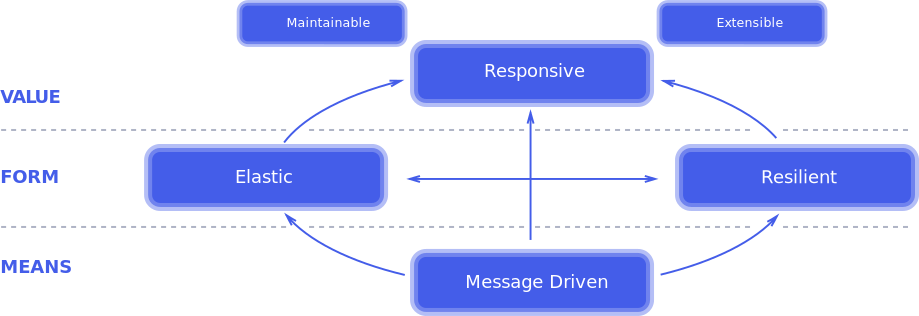
\includegraphics[width=\linewidth, scale=0.4]{images/reactive-traits.png}
    \end{figure}

    As figure \ref{fig:reactive-value} suggests, designing and implementing a distributed system in reactive style
    has the following benefits: easier to maintain, easier to change and higher responsiveness.

    So in summary, a reactive system consists of isolated components communicating using asynchronous non-blocking message passing.

    An ideal reactive system conforms to ACID2\cite{reactive-microsystems}.
    ACID2 is the counterpart of ACID in transactional databases.
    So instead of atomicity, consistency, isolation, durability, ACID2 is:
    \begin{itemize}
        \item \textbf{Associative:} Messages can be grouped together, using a key for example.
        \item \textbf{Commutative:} The order at which messages arrive to components does not affect the desired
        outcome.
        \item \textbf{Idempotent:} Components of system should receive a message more than once, they act as if message arrived only once.
        \item \textbf{Distributed:} .
    \end{itemize}

    A reactive system, specially when conforming to ACID2, has potential to scale out very easy to a very a high extent.

    When it comes to replication of data over components in a reactive system, in case consistency matters, order of
    messages becomes important.
    Order at which messages arrive has a logical time aspect which is important for achieving occasional consistency.
    It is very challenging for a distributed system to be strongly consistent.
    So if it is acceptable to relax the requirements to occasional/eventual consistency, a reactive system in which
    order of messages are reserved works well.

    The style with which messages are produced has a direct effect on system design and implementation.
    A message can be a query (what is X), an event (X has happened), a command (do X) and an update (X is 232 now).
    The preferred message semantic in reactive systems is \textbf{event}s.
    An event represent something that has happened in the past, an immutable truth.
    Such events can be published into a queue reserving their order.
    System components can subscribe to the queue and update their own image of the world (state) according to the
    events that has happened.

    In order to achieve such a system design, events should be considered first in the design rather than the domain.
    Verbs first rather than nouns, what happened vs what exists, immutable fact vs cumulative knowledge.

    \subsection{Microservices}
    Once upon a time the whole software, an information system for example, was one process deployed manually on a big
    physically available machine.
    This software was maintained by a big team in one code base.
    To change any part of it, was a headache to make sure even the smallest change will not break the whole software.
    Everything was tightly coupled after all.
    It was all about code re-use.
    If developers managed to change it properly, building the code took hours and forget about how long it took to
    run the tests (if there was any of course).
    After manually deploying the executable artifact into a physically available server in the corner of office, an
    equal sign forgotten in a loop condition, brought the whole service down 11 pm same day.
    Manager panics, wakes every developer who can, with hope of a hot fix.

    Hot fix applied, everyone back to sleep, customers are happy.
    If fact so happy that they invite their friends to use the service.
    More clients, more money, great.
    Too good to be true though.
    14 pm next day, number of users using the service simultaneously rockets to outside range of available resources.
    CPU usage is 100 percent, no free memory left on the machine and only one out of 10 user is actually getting
    service instead of just looking at loading bar.

    Developers run around city to find RAMs with bigger capacity as a temporal solution.
    IT people start to think about assembling a more powerful server with all brand-new more powerful hardware.

    Those days are gone due to adoption of cloud technologies combined with microservices.

    \paragraph{Microservices} is an architectural style in which software is divided into some small components
    called services.
    Those (micro)services communicate with each other and serve the overall purpose of software.
    Each service is maintained by a special team, has its own code base, has its own database, exposes its own APIs, is
    tested independently, is packaged separately and is deployed as a separate process.

    The less these services share, the better.
    Decoupling services as much as possible is an important aspect of microservices.
    Because for example, the less services are dependent on each other, the easier they can be changed.

    So now that software is developed into microservices, each microservice can be changed independently by the
    team responsible for maintaining it, deployed separately after a short build and test process.
    A bug in one of the services can not bring the whole system down as well.
    When load on one of the microservices increases, more instances of it can be easily deployed (scale out).
    And hopefully instead of deploying executable artifact into a physically available machine in the corner of
    office, microservices are packaged as docker images and deployed into a container orchestration tool provided as
    a managed cloud service.

    Of course turning a monolith into a distributed system brings all the challenges of distributed systems with it.
    Having data spread around different services makes strong consistency very hard to achieve.
    Load balancing between available instances of each service is something new to deal with.
    Monitoring of and communication between services requires special attention.
    And so on.
    In order to solve the mentioned challenges and much more, best practices, design patterns, architectural patterns
    and tools become handy.
    System designers and developers select a sub set of these helps based on the functional and non-functional
    requirements of their system, size of their organization and other relevant factors.
    API gateway, Service registry, Distributed tracing, CQRS, Saga are some popular examples.
    \cite{microservice-architecture} \cite{microservices-pitfalls} \cite{microservices}

    \subsection{Stream processing}
    Stream processing refers to a special style of reactive systems.
    It is also equivalent to data flow programming in which a graph of operators exists.
    These operators receive events as a result of work of other operators, process them and produce other events.
    These events represent immutable facts, something that has happened.
    The order at which events arrive to the next operator matters;
    so usually in stream processing systems, publish-subscribe pattern implemented using some sort of queue,
    journal, commit log or topic.
    \cite{flink} \cite{fast-data-archs}

    The foundation of a stream processing pipeline is its data flow graph.

    \subsubsection{Data flow graph}
    Data flow graph is a useful tool to express and study how data is flown in a stream processing system.
    There are two type of data flow graphs: \textbf{logical} and \textbf{physical}.
    In a logical data flow graph nodes represent \textbf{operators} like sum, count, filter and aggregate.
    It does not give any information about deployment.
    On the other hand, a physical data flow graph illustrates how exactly the pipeline looks when deployed.
    Like how many instances of each \textbf{task} should be deployed.
    Task is equivalent of operator but in physical data flow graph.
    We implement an operator and deploy it as some tasks.
    Similar to implementing a microservice and deploying some instances of it.

    \begin{figure}[ht]
        \caption{Example of physical data flow graph. Taken from \cite{flink}}
        \label{physical-data-flow-graph-example}
        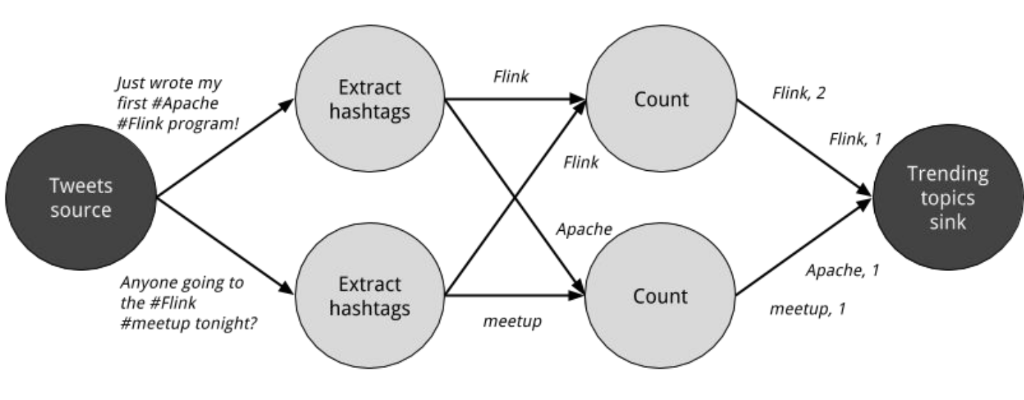
\includegraphics[width=\linewidth, scale=0.6]{images/physical-data-flow-graph.png}
    \end{figure}

    Graph \ref{physical-data-flow-graph-example} shows an example of a physical data flow graph with 6 tasks (3
    operators).
    This pipeline counts occurrences of each hashtag in a stream of tweets which includes following operators:

    \begin{itemize}
        \item A source that brings tweets into the stream processing pipeline
        \item A processor that extracts hashtags
        \item A stateful processor that counts occurrences of each hashtag
        \item A sink that represents end of this pipeline which receives realtime count of each hashtag. It might
        save results in a file or publish them to another system.
    \end{itemize}

    \subsubsection{Parallelism}
    There are two types of parallelism is stream processing systems:

    \paragraph{Task parallelism}
    Tasks from different operators process same data.
    Imagine having a stream of tweets.
    One operator extract hashtags, another one extracts mentions and maybe another counts number of words in each
    tweet.

    \paragraph{Data parallelism}
    Tasks from same operator process different data.
    The data (event) in the topics of pipeline is in key:value format.
    Data with same key ends up in the same task unless the corresponding task stops working (re-balancing).
    Data parallelism is achievable by technics like partitioning of topic which is implemented by tools like Kafka.
    Data parallelism is basically equivalent to concept of scaling out in microservices terminology (scaling
    horizontally).

    \subsubsection{Latency}
    Latency, in stream processing systems, is defined as the time takes for ONE event to be processed.
    In an ideal stream processing system, the latency reflects the actual processing work on the events.
    Which means events don't wait to be processed.
    In other words events get processed as soon as they arrive.
    \textbf{95th-percentile latency value of 10ms`} is an example of expressing latency in stream processing system.
    It means 95 percent of events are processed within 10 ms.
    Obviously, the lower the latency, the better.

    \subsubsection{Throughput}
    Throughput, in stream processing systems, depends on both latency and input rate.
    So low throughput doesn't necessarily mean high latency.
    A better metric is \textbf{peak throughput} which shows the limit on the performance of system at maximum load.
    When system reaches peak throughput, increasing input load, will actually reduce throughput and can even lead to
    data loss (due to buffer overflow).

    \subsubsection{Operations}
    There are two types of operations:
    \textbf{Stateless} operations like filter and map are not concerned with past.
    They are easier to scale and more resilient.
    While \textbf{stateful} operations keep a snapshot of past (state).
    The state may mutate after processing each event.
    Operations like sum, count, average and aggregate are stateful.
    Such operations are harder to scale.
    The hardship comes from the fact that apart from scaling out the tasks, the state part assinged to each task need
    to become co-located for the task.
    It brings challenges like the best partitioning policy and correct key selection.
    For example when partitioning geospatial data partitioning policy may differ based on the use case.

    \section{Underlying tools}
    In this section we describe some of many technologies which taken into action in order to make FenceX possible.
    The explanation won't exceed a simple introduction since detailed information goes beyod context of this thesis.

    \subsection{Kafka}
    Kafka\cite{kafka} is an event streaming tool.
    It is a distributed implementation of journal (commit log).
    Main components in the Kafka ecosystem are: a cluster of servers (brokers) and clients (event producers and consumers).
    The broker is written in Scala while client libraries are available in variety of programming languages.

    Kafka is one of the famous go to option when an architecture relies on publish subscribe pattern.
    It has a concept called \textbf{topic} which is a durable journal (a queue).
    The subscribers to the topic can be grouped for load distribution purposes.
    Each topic can be partitioned so that each group member subscribes to a partition of a topic.
    Publisher is responsible for selecting the partition to which an event should be published.

    Events in each partition can be replicated over cluster of Kafka brokers for availability purposes.

    \textbf{only once} and \textbf{at least once} are the available quality of services that Kafka provides.

    When using Kafka, a set of APIs are available to use: producer, consumer, admin, connect and \textbf{Kafka Streams}.
    There are basically way for interacting with broker and their name exposes their functionality.

    \subsubsection{Kafka Streams}
    Kafka Streams\cite{kafkaStreamsJoins} is a JVM languages compatible library which allows for publishing
    data into and reading data from a Kafka cluster in form of stream processing operations.
    A microservices can just has it as a library, connects to Kafka, defines an operation like \textbf{filer} or
    \textbf{aggregate} and becomes a node in a stream processing pipeline, a node in a data flow graph.
    The definition of such operations starts with creating a KStream on top of a topic.
    Each event in the topic, will be an event in the stream.

    As opposed to other Kafka APIs like producer that are stateless, Kafka Streams supports both stateless and
    stateful operations.
    For stateful operations, Kafka Streams ask for defining a KTable.
    KTable is a key:value table which is essentially backed by a kafka topic as source of truth.
    However, for ease of accessibility, the data in the topic gets loaded into a database which is RocksDB by default.
    In case of FenceX, in poll leg, we have used H2 in an in-memory fashion.

    Kafka Streams concept of KTable is not much different from concept of a Table in a traditional database.
    So it is not unexpected for it to allow for join operations.
    A join operation can be defined between: two KStreams, two KTables, a KTable and a KStream.
    In FenceX we have joined a KTable with a KStream.
    Which means each time an event comes to the stream, a function will be called with two inputs: the event and the
    key:value record in the KTable with the same key as the event.

    Kafka Streams also supports concepts like event time which allows for defining windowing operations.
    A use case could be counting number of clicks on a link during each 5 minutes window when each click results in
    an event.

    \subsection{Docker}

    \subsection{Nomad}

    \chapter{System deployment}
    The deployment configuration for FenceX microservices in production depends on the exact needs of business.
    It is also always limited to the hardware resources available, like any other software.
    During evaluation of FenceX for this thesis we had access to 4 virtual machines with the following resources
    available to them.

    \begin{table}[h!]
        \centering
        \begin{tabular}{|c|c|c|c|}
            \hline
            Server  & CPU CORES & RAM(GB) & Main responsibility \\
            \hline
            server1 & 8         & 16      & Master keeper       \\
            server2 & 4         & 8       & Nomad worker node   \\
            server3 & 4         & 8       & Nomad worker node   \\
            server4 & 4         & 16      & Benchmarking        \\
            \hline
        \end{tabular}
        \caption{Virtual machines used in evaluation of FenceX and their overall responsibility}
        \label{table:vms}
    \end{table}

    Figure \ref{fig:infrastructure} illustrates how FenceX deployment looks from infrastructure point of view in a
    evaluation scenario.
    The only difference compared to other possible evaluation scenarios is the number of deployed instances of FenceX
    microservices, realtime-fencing for example.

    \begin{figure}[h!]
        \centering
        \caption{FenceX infrastructure setup for evaluation}
        \label{fig:infrastructure}
        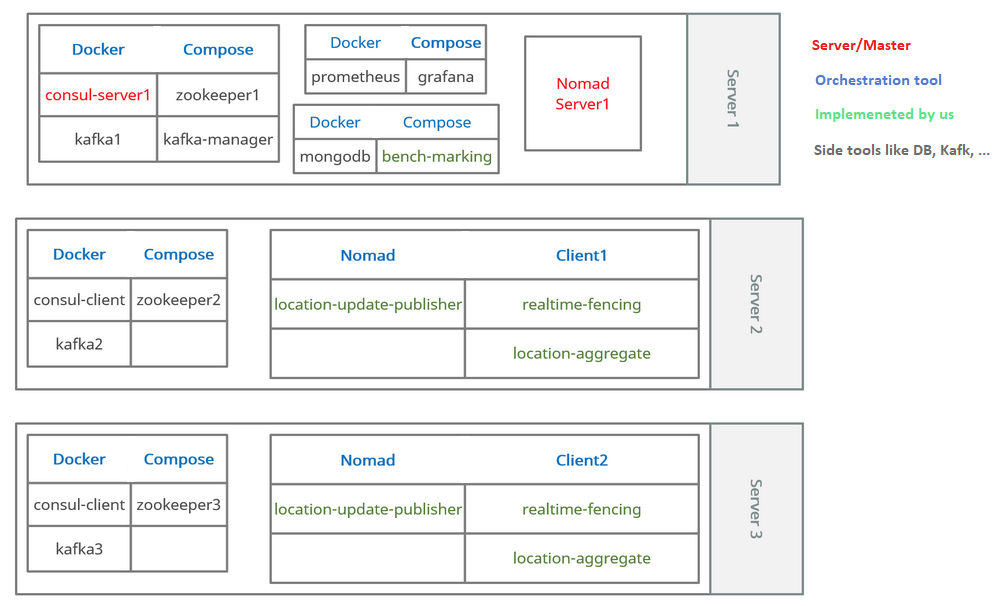
\includegraphics[scale=0.6]{images/Infrsutracture.png}
    \end{figure}

    Figure \ref{fig:infrastructure} does not include server4 since that server only runs an instance of bench-marking
    application which is not part of the FenceX solution package.
    Nevertheless, we have deployed another instance of bench-marking into server1 as well;
    since getting high throughput out of bench-marking applications is very expensive in terms of resources.

    Tools like Kafka and Zookeeper are deployed as docker containers to keep the setup phase of evalution easier.
    In production, they are usually deployed directly on separate hosts.
    However, for FenceX evaluation we have used docker-compose on top of docker to manage the life cycle of docker
    containers in an easy and convenient way.

    It is also important to note that FenceX had 4 major Kafka topics.
    \textit{fence\_event\_log, location-aggregate-mover-in-memory-state-store-changelog, mover-position-updates,
        realtime-fencing-fence-state-store-changelog}.
    All of these topics were configured to have 3 replicas and 12 partitions.
    These numbers are selected corresponding to the overall available resources.
    The process of selecting them correctly is out of the context of this thesis.
    The important factor however is to have a high enough replication factor to achieve availability (3 at least) and
    high enough number of partitions to avoid idle subscribers.

    \paragraph{}
    In terms of bandwidth, between virtual machines hosting FenceX infrastructure during evaluation, in both
    directions we observed numbers more than 3Gbps.
    However, since the process of producing load was computationally expensive, we did not even get close to saturating
    the available bandwidth.

    \paragraph{}
    After preparing the infrastructure, Nomad calculated available resources to the applications that will be
    deployed into worker nodes as 16670 MHz of computation power and 16 GB of memory.

    \chapter{Experiments and validation}
    In this chapter we explain the process and results of evaluating FenceX.
    This process consists of many experiments with different setup and goals.
    Each experiment had a preparation phase, execution, observation and finally conclusion.

    \subsection{Benchmarking application}
    Before diving into the test cases, it is worth the effort to explain how bench-marking application works and what
    functionalities it provides.

    Generally speaking it is a microservice similar to other services in FenceX.
    It registers itself into Consul and has HTTP APIs.
    It is based on spring-webflux\cite{webflux} reactive stack in order to handle IO better.
    The role of bench-marking is to imitate the behaviour of real world mover location report publishers,
    smartwatches or car gps modules for example.

    bench-marking has a dataset of real taxi trips.
    Each trip has an (anonymized) ID, a set of location reports (points), a geospatial circle (fence) drawn around one
    of those points.
    The points are in form of coordinates (latitude, longitude) and the fences are WKT strings.
    Each trip has an average of 17 points and in total around 500 trips are in the database.

    \paragraph{}
    bench-marking can send HTTP requests to realtime-fencing and define fences for movers.
    For simplicity mover ID will the trip ID.

    \paragraph{}
    bench-marking can send HTTP requests to location-update-publisher and report coordinates for each trip.
    The result in FenceX will be a stream of location updates published into the pipeline.

    \paragraph{}
    bench-marking can send HTTP requests to location-aggregate and query its location database against the fence
    defined for each trip.

    bench-marking can do operations mentioned above for all the trips repeatedly very fast in order to push a
    stressful load of inputs into the FenceX pipeline.
    It can also keep the size of load low while keeping it ongoing (non-stop) over time.

    It appeared that producing stressful loads of HTTP request or ongoing flows of them is a very expensive operation
    in terms of memory and CPU usage.
    Mostly during our evaluations the bottleneck to throughput was our input rate.


    \section{Evalution of system throughput}
    In this section we go over the experiments we have conducted in order to not only stress test FenceX but also
    calculate the peak throughput based on available resources.
    Throughput is a direct factor of input rate both for on demand poll style operations and realtime push style ones.
    For on demand style, the input rate is the number of HTTP requests (query by fence) per second that system receives.
    For realtime operations, the input rate is the number of location reports arrive at system per second.
    As mentioned previously, for each setup, exists a threshold for input rate above which throughput won't go any
    higher by increasing input.

    \paragraph{}
    In order to calculate the throughput in each experiment, we use a combination of tools, Prometheus and
    Grafana\cite{grafana}.
    Prometheus is a time series database that polls different types of metrics out of each of FenceX microservices on
    a frequent basis.
    Grafana is a visualization tool that reads metric data from Prometheus and illustrates it into a variety of graphs.
    The metrics can be general like CPU usage or number of JVM threads.
    They can also be custom to each application like number of fence-point intersection calculations.
    Using this setup, we created realtime graphs that shows pull and push throughput of FenceX in addition to other
    information like push and poll input rate.
    Thanks to that, we do not need to calculate the throughput after each experiment.
    We can just have a look at the corresponding graphs during execution of test scenarios in order to see the realtime
    value of throughput and input rate.

    \paragraph{}
    During evaluation for both legs of FenceX, we expect the highest throughput that we will observe to be higher
    than corresponding throughput achieved by \cite{Nechifor_Comnac_2013} and
    \cite{Cirillo-Jacobs-Martin-Szczytowski-2014}.
    We will provide a more detailed comparison at the end of this section.

    \subsection{Push leg}
    Push throughput evaluation scenario:
    \begin{itemize}
        \item[1-] Define fences for movers using all the trips in the bench-marking application database.
        \item[2-] Send a shocking stream of location reports into the FenceX.
        \item[3-] Check the throughput.
        \item[4-] Repeat the experiment after changing the deployment configuration and input rate pattern. (Maybe add
        more instances or add more CPU) until finding peak throughput and/or a possible upper bound for throughput.
    \end{itemize}

    \subsubsection{Experiment 1}
    \begin{table}[h!]
        \centering
        \begin{tabular}{|c|c|c|c|}
            \hline
            Application               & number of instances & CPU(MHz) & RAM(MB) \\
            \hline
            location-update-publisher & 4                   & 500      & 500     \\
            location-aggregate        & -                   & -        & -       \\
            realtime-fencing          & 4                   & 700      & 800     \\
            \hline
        \end{tabular}
        \caption{Experiment 1 deployment view}
        \label{table:ex1-dv}
    \end{table}

    Table \ref{table:ex1-dv} shows, for experiment 1, how many instances of each FenceX microservices we have initially
    deployed in addition to the amount of resources we have assigned to each.
    The row in table \ref{table:ex1-dv} with no values corresponds to a microservice which does not relate to the
    experiment 1.
    After successful deployment, we followed the previously mentioned scenario.
    The following figures illustrate how input rate and throughput have changed during each repetition of experiment 1
    with different input rate patterns.
    It is important to note that the pattern at which input rate changes, which differs among repetitions, is not of
    relevance to system throughput experiments.
    What matters in these experiments is that if throughout follows the input rate pattern in addition to the highest
    achieved throughput.

    \begin{figure}[h!]
        \centering
        \caption{FenceX push throughput ex1-1}
        \label{fig:ex1-1}
        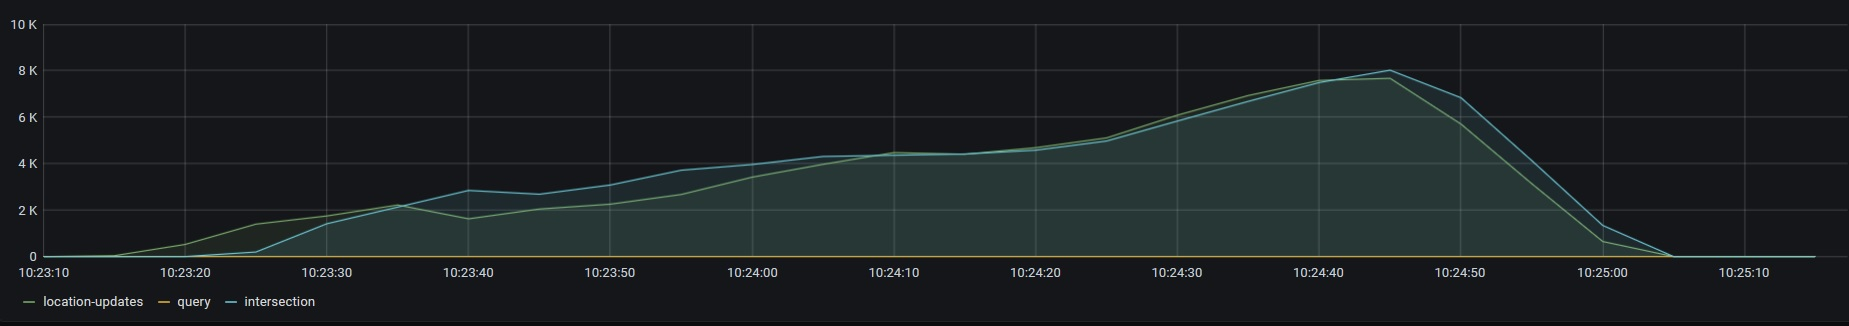
\includegraphics[width=\linewidth, scale=2]{images/evaluation/ex1-benchmarking(15,6).png}
    \end{figure}

    \begin{figure}[h!]
        \centering
        \caption{FenceX push throughput ex1-2}
        \label{fig:ex1-2}
        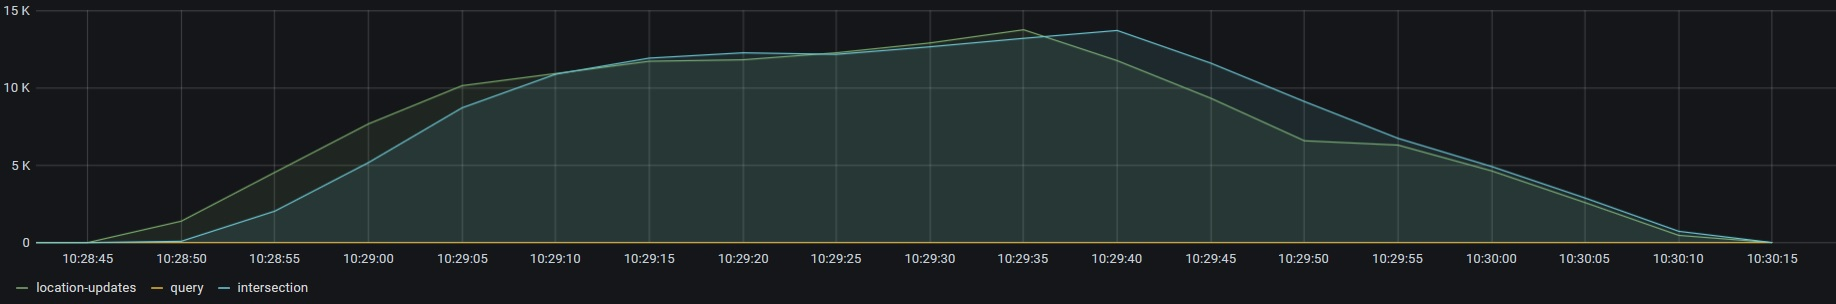
\includegraphics[width=\linewidth, scale=2]{images/evaluation/ex1-benchmarking(19,7).png}
    \end{figure}

    \begin{figure}[h!]
        \centering
        \caption{FenceX push throughput ex1-3}
        \label{fig:ex1-3}
        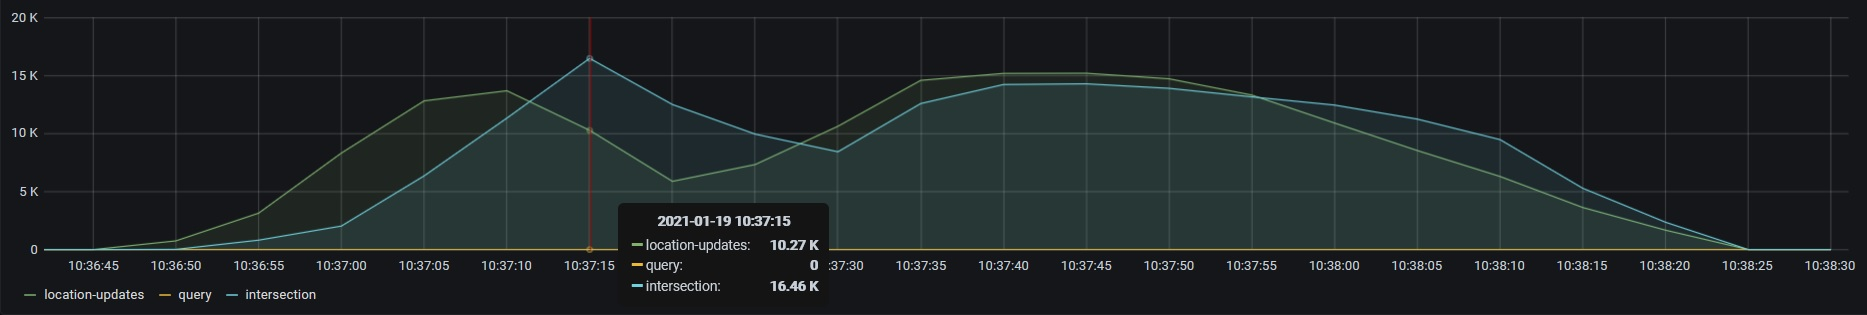
\includegraphics[width=\linewidth, scale=2]{images/evaluation/ex1-benchmarking(22,9).png}
    \end{figure}

    \begin{figure}[h!]
        \centering
        \caption{FenceX push throughput ex1-4}
        \label{fig:ex1-4}
        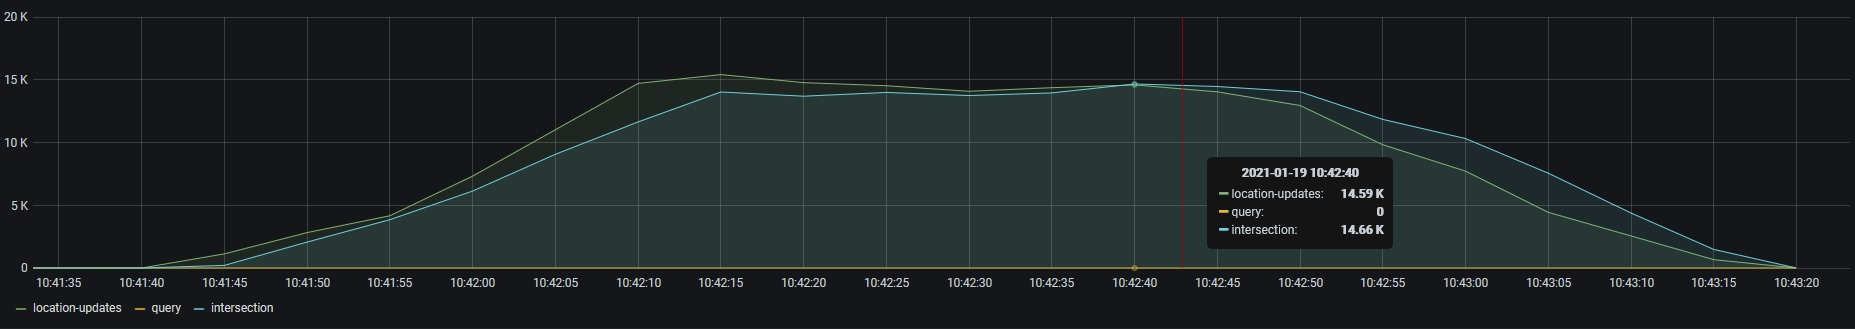
\includegraphics[width=\linewidth, scale=2]{images/evaluation/ex1-benchmarking(23,10).png}
    \end{figure}

    The figures \ref{fig:ex1-1}, \ref{fig:ex1-2}, \ref{fig:ex1-3} and \ref{fig:ex1-4} illustrate input rate
    (location-updates per second) with green line and push throughput (number of fence-point intersection
    calculations per second) with the blue line.
    These figures show that when we tried different input rates (ranging from 8k/s to 15k/s), the throughput was
    following the change patterns in input rate.
    Also, throughput were mainly always as high as input rate.
    The highest input rate we managed to produce during these experiments was around 15K location updates per second
    and FenceX just managed to handle it very well with the given deployment setup.

    \clearpage

    \subsubsection{Experiment 2}
    \begin{table}[h!]
        \centering
        \begin{tabular}{|c|c|c|c|}
            \hline
            Application               & number of instances & CPU(MHz) & RAM(MB) \\
            \hline
            location-update-publisher & 5                   & 400      & 700     \\
            location-aggregate        & -                   & -        & -       \\
            realtime-fencing          & 5                   & 400      & 700     \\
            \hline
        \end{tabular}
        \caption{Experiment 2 deployment view}
        \label{table:ex2-dv}
    \end{table}

    Table \ref{table:ex2-dv} shows, for experiment 2, how many instances of each FenceX microservices we have
    deployed in addition to the amount of resources we have assigned to each.
    Compared to experiment 1, 1 more instance of each related microservice is deployed but with slightly lower
    computation power available to each.
    The row in table \ref{table:ex2-dv} with no values corresponds to a microservice which does not relate to the
    experiment 2.
    The following figure illustrates how input rate and throughput have changed during experiment 2.

    \begin{figure}[h!]
        \centering
        \caption{FenceX push throughput ex2}
        \label{fig:ex2}
        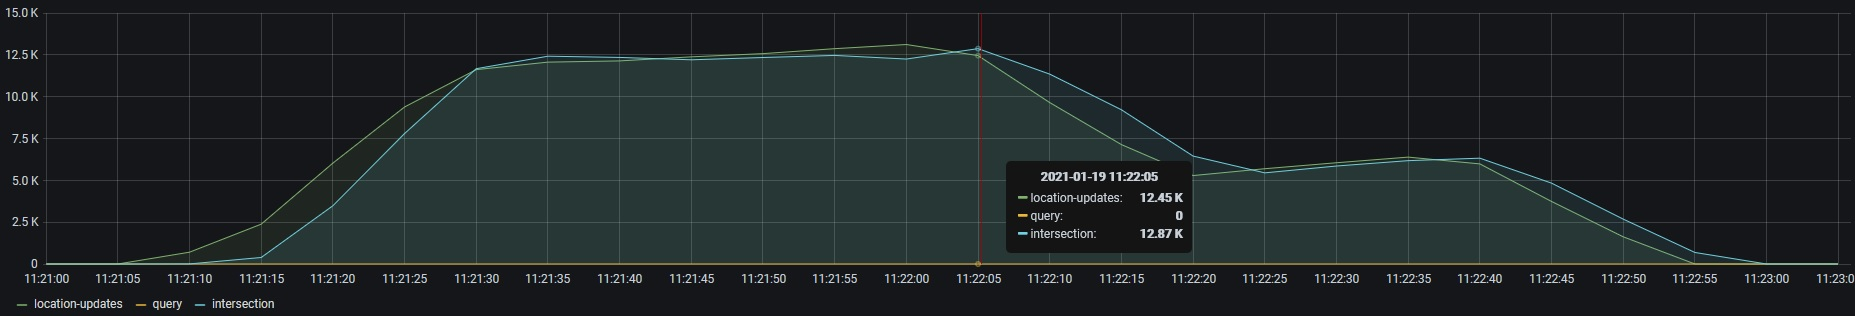
\includegraphics[width=\linewidth, scale=2]{images/evaluation/ex2-benchmarking(24,10).png}
    \end{figure}

    The figure \ref{fig:ex2} can be read in the same way as figures in experiment 1 (figures \ref{fig:ex1-1} for
    example).
    We have deployed one more instance of relevant microservice plus changing the input rate pattern.
    The throughput again followed the input pattern.

    \subsubsection{Conclusion of system throughput evaluation}
    So far the bottleneck is input rate which is limited by our physical resources available to bench-marking
    application.
    We can clearly see in the graphs that regardless of setup, push throughput (intersections/second) follows pretty
    much the exact pattern of changes in input rate (location updates/second).
    So there is no point in continuing push throughput experiments with current available hardware power.
    The highest throughput observed for push leg so far therefore is ~15k/s.

    \clearpage

    \subsection{Poll leg}
    Poll throughput evaluation scenario:
    \begin{itemize}
        \item[1-] Send many location updates to FenceX using all the trips in the bench-marking application database.
        \item[2-] Send a shocking load of queries (query by fence) to FenceX.
        \item[3-] Check the throughput.
        \item[4-] Repeat the experiment after changing the deployment configuration. (Maybe add more instances or add
        more memory) until finding peak throughput and/or a possible upper bound on throughput.
    \end{itemize}

    \subsubsection{Experiment 3}
    \begin{table}[h!]
        \centering
        \begin{tabular}{|c|c|c|c|}
            \hline
            Application               & number of instances & CPU(MHz) & RAM(MB) \\
            \hline
            location-update-publisher & 4                   & 500      & 500     \\
            location-aggregate        & 2                   & 2500     & 3200    \\
            realtime-fencing          & -                   & -        & -       \\
            \hline
        \end{tabular}
        \caption{Experiment 3 deployment view}
        \label{table:ex3-dv}
    \end{table}

    Table \ref{table:ex3-dv} shows, for experiment 3, how many instances of each FenceX microservices we have initially
    deployed in addition to the amount of resources we have assigned to each.
    The row in table \ref{table:ex3-dv} with no values corresponds to a microservice which does not relate to the
    experiment 3.
    The following figure illustrates how input rate and throughput have changed during experiment 3.

    \begin{figure}[h!]
        \centering
        \caption{FenceX poll throughput ex3}
        \label{fig:ex3}
        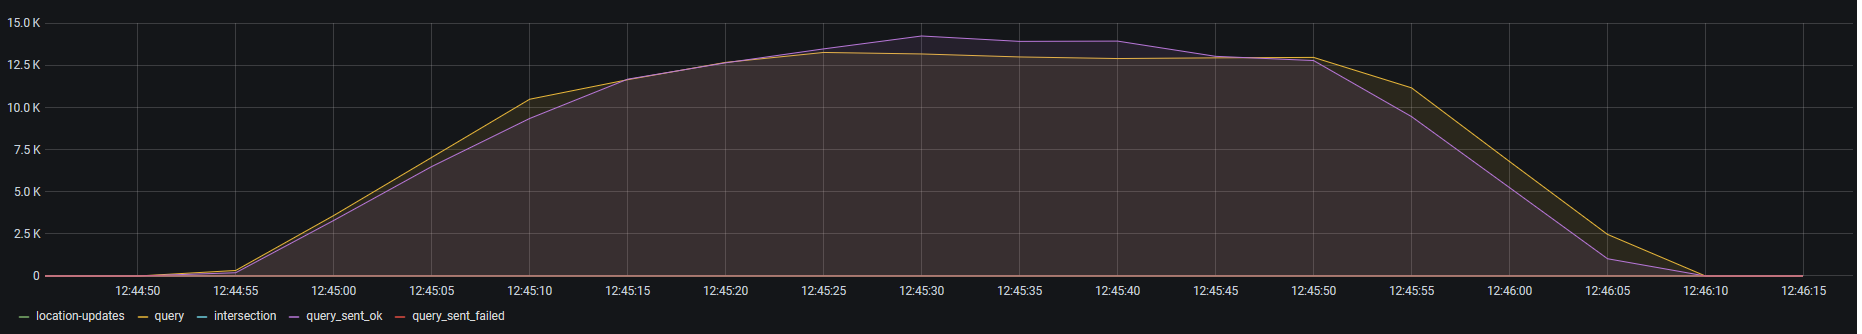
\includegraphics[width=\linewidth, scale=2]{images/evaluation/ex3-benchmarking(16,9).png}
    \end{figure}

    Figure \ref{fig:ex3} illustrates input rate (queries sent successfully per second) with purple line and poll
    throughput (number of queries answered without error) with the yellow line.
    In this experiment, the input rate was around 12k/s at highest which is handled well by 2 rather rich instances of
    location-aggregate.

    \clearpage

    \subsubsection{Experiment 4}
    \begin{table}[h!]
        \centering
        \begin{tabular}{|c|c|c|c|}
            \hline
            Application               & number of instances & CPU(MHz) & RAM(MB) \\
            \hline
            location-update-publisher & 4                   & 500      & 500     \\
            location-aggregate        & 2                   & 2700     & 2700    \\
            realtime-fencing          & -                   & -        & -       \\
            \hline
        \end{tabular}
        \caption{Experiment 4 deployment view}
        \label{table:ex4-dv}
    \end{table}

    Table \ref{table:ex4-dv} shows, for experiment 4, how many instances of each FenceX microservices we have
    deployed in addition to the amount of resources we have assigned to each.
    Compared to experiment 3, we have only changed the available resources to location-aggregate.
    The row in table \ref{table:ex4-dv} with no values corresponds to a microservice which does not relate to the
    experiment 4.
    The following figures illustrate how input rate and throughput have changed during experiment 4 while applying
    different patterns of input.

    \begin{figure}[h!]
        \centering
        \caption{FenceX poll throughput ex4-1}
        \label{fig:ex4-1}
        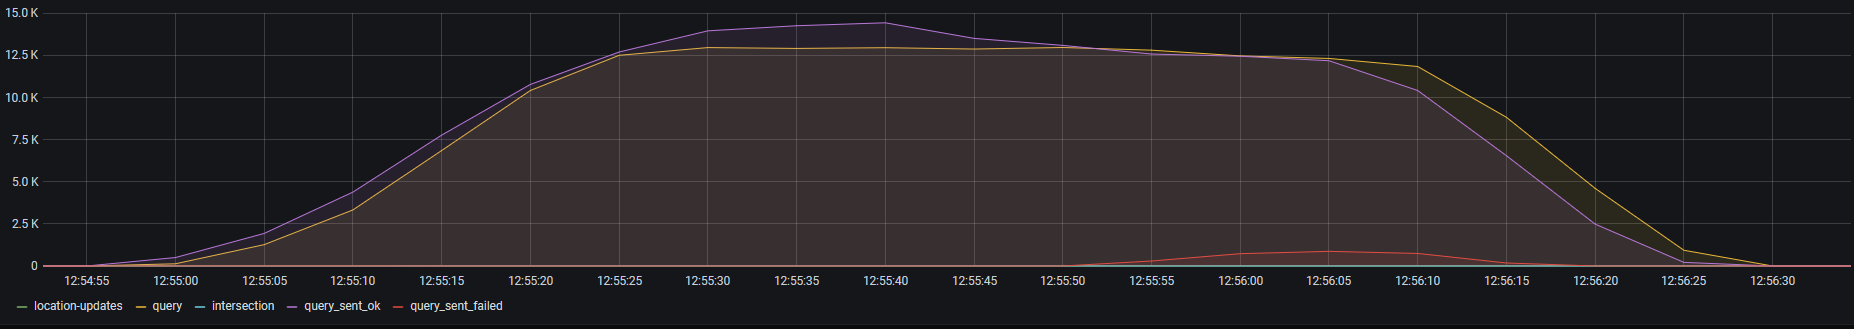
\includegraphics[width=\linewidth, scale=2]{images/evaluation/ex4-benchmarking(19,10).png}
    \end{figure}

    \begin{figure}[h!]
        \centering
        \caption{FenceX poll throughput ex4-2}
        \label{fig:ex4-2}
        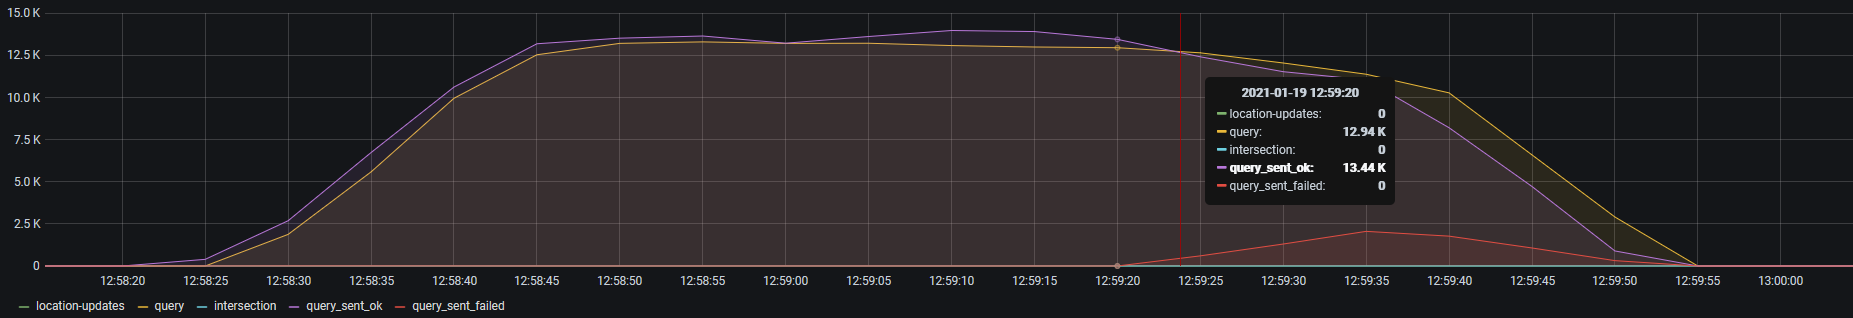
\includegraphics[width=\linewidth, scale=2]{images/evaluation/ex4-benchmarking(22,10).png}
    \end{figure}

    Both figure \ref{fig:ex4-1} and \ref{fig:ex4-2} can be read similarly to the graphs from experiment 3.
    Comparing to experiment 3, in experiment 4 we changed the available resources to poll leg plus changing the input
    rate pattern.
    The change in the input pattern is subtle however.
    In this experiment, the input rate was around 12k/s at highest which is handled well by poll leg of FenceX.

    \subsubsection{Conclusion of poll throughput evaluation}
    Experiments 3 and 4 show that we have failed to increase the input rate as we progressed.
    Although the CPU usage on location-aggregate instances peaked to 100 percent during these experiments,
    again the bottleneck was input rate which is limited by our physical available resources.
    We can clearly see in the graphs that regardless of setup, poll throughput (queries/sec) follows pretty
    much the exact pattern of changes in input rate (queries sent/sec).
    So there is no point in continuing poll throughput experiments with current available hardware.
    However, the highest input rate we managed to produce during these experiments was in the range of [12-13]k queries
    per second which FenceX just managed to handle very well.


    \section{Availability}
    In this section we cover the experiments we have conducted in order to test availability of FenceX.
    We evaluate availability by observing the throughput of system under non optimal conditions.
    In order to test FenceX for availability, roughly speaking, we start an ongoing load or stream of input.
    Once throughput becomes stable, we restart one of the instances of involved microservices.
    The overall expectation is that during the restart, until the service becomes up and running again, the throughput
    goes down and afterward goes up again to the previous value.
    The main factor affecting the time takes until the service is up and running again is re-balancing.
    Kafka topics have consumer groups.
    Each member of a group, listens to a subset of partitions of that topic.
    This essentially results in data parallelism.
    A topic can have multiple groups listening to it which essentially is foundation of task parallelism.
    Re-balancing happens when one of the group members becomes unhealthy and stops subscribing to its assigned
    partitions.
    At this moment, other healthy group members should take over the dangling partitions.
    The processes of reassigning the dangling partitions to healthy subscribers is called re-balancing.
    The time a possibly successful re-balancing takes depends on the number of partitions and available
    healthy subscribers.
    So the time takes until throughput goes back to previous value is also not fixed.

    Please note that after a restart, there will be two re-balancings.
    One once the service under restart goes down and another once it comes back up and running.
    If the remaining services after first re-balancing, had enough resources available, the throughput won't change
    that much.
    Specially for lower input loads.

    \subsection{Push leg}
    Push leg availability evaluation scenario:
    \begin{itemize}
        \item[1-] Define fences for movers using all the trips in the bench-marking application database.
        \item[2-] Start an ongoing stream of location report toward FenceX.
        \item[3-] Wait until throughput becomes stable.
        \item[4-] Restart one of the instances of realtime-fencing.
        \item[5-] Assert that throughput drops.
        \item[6-] Wait until successful re-balancing.
        \item[7-] Assert that throughput is back to previous value.
        \item[8-] Repeat the experiment with difference of restarting two instances instead of one.
    \end{itemize}

    \clearpage

    \subsubsection{Experiment 5}
    \begin{table}[h!]
        \centering
        \begin{tabular}{|c|c|c|c|}
            \hline
            Application               & number of instances & CPU(MHz) & RAM(MB) \\
            \hline
            location-update-publisher & 5                   & 400      & 700     \\
            location-aggregate        & -                   & -        & -       \\
            realtime-fencing          & 6                   & 400      & 800     \\
            \hline
        \end{tabular}
        \caption{Experiment 5 deployment view}
        \label{table:ex5-dv}
    \end{table}

    Table \ref{table:ex5-dv} shows, for experiment 5, how many instances of each FenceX microservices we have initially
    deployed in addition to the amount of resources we have assigned to each.
    The row in table \ref{table:ex5-dv} with no values corresponds to a microservice which does not relate to the
    experiment 5.
    The following figures illustrate how input rate and throughput have changed during repetitions of experiment 5.
    Each repetition was with different input load pattern.
    They also show how (and when) number of deployed instances of related microservices has changed during this
    experiment.

    \begin{figure}[h!]
        \centering
        \caption{FenceX push leg availability ex5-1}
        \label{fig:ex5-1}
        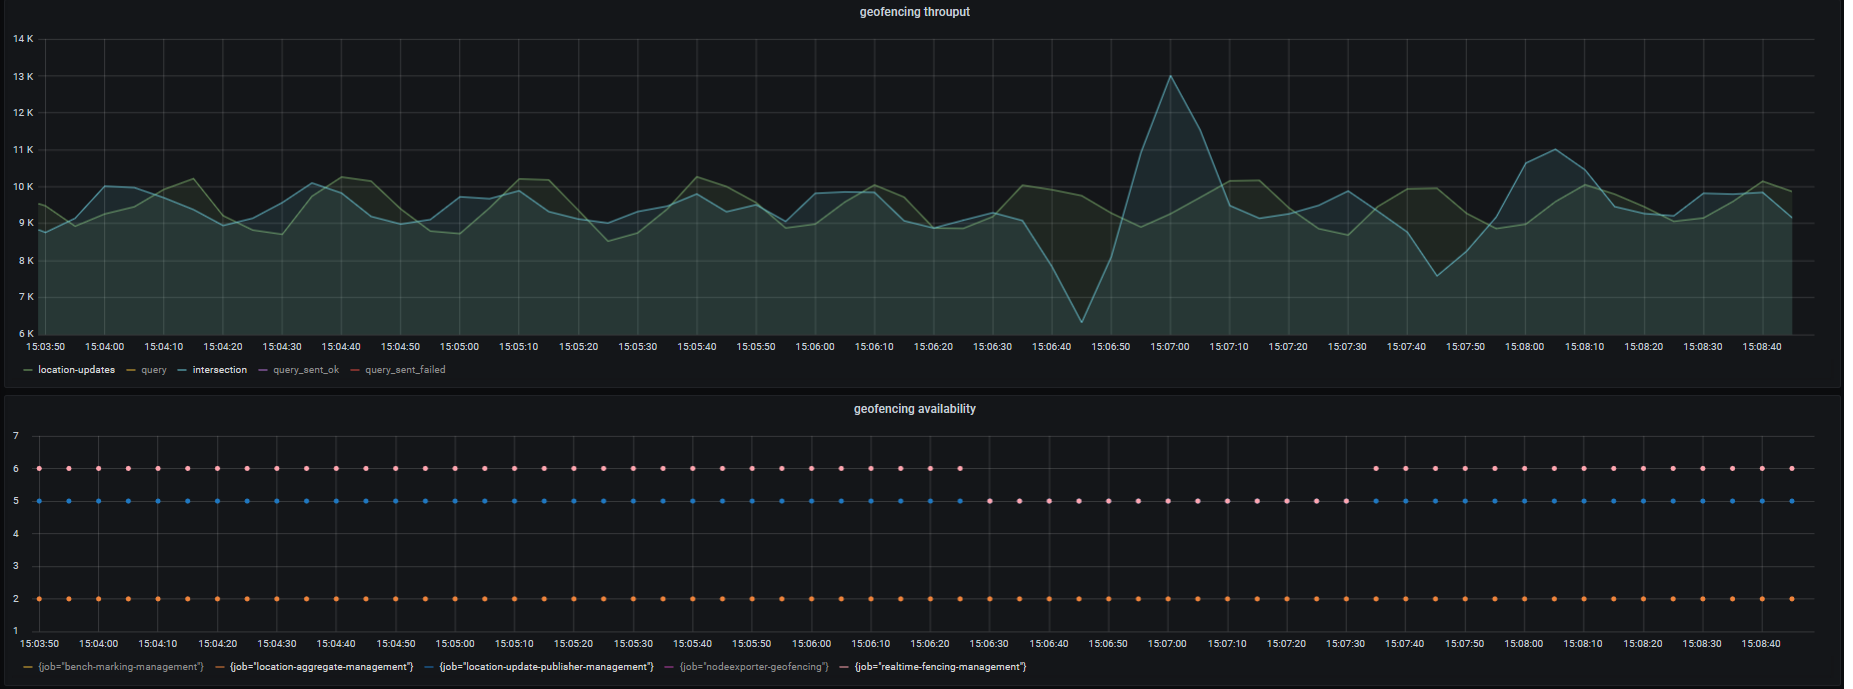
\includegraphics[width=\linewidth, scale=0.4]{images/evaluation/ex5-benchmarking-ongoing-2per6sec.png}
    \end{figure}

    \begin{figure}[h!]
        \centering
        \caption{FenceX push leg availability ex5-2}
        \label{fig:ex5-2}
        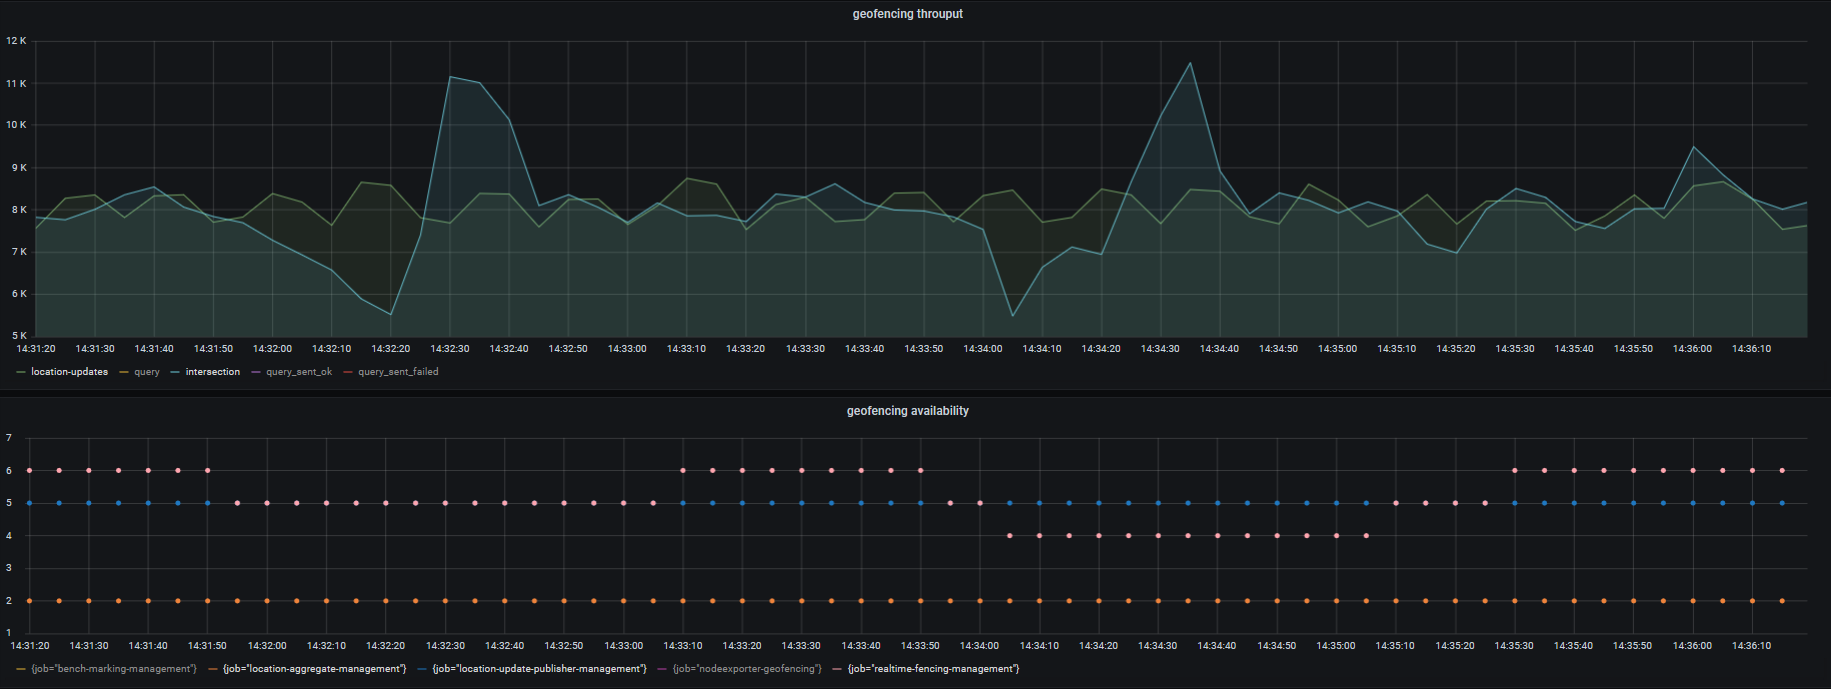
\includegraphics[width=\linewidth, scale=2]{images/evaluation/ex5-benchmarking-ongoing-2per7sec.png}
    \end{figure}

    In figures \ref{fig:ex5-1} and \ref{fig:ex5-2}, blue line represents the push throughput.
    Green line illustrates the ongoing input stream of location updates and pink point shows
    number of up and running instances of realtime-fencing.

    As you can see in figures \ref{fig:ex5-1} and \ref{fig:ex5-2}, there are points in the timeline at which number of
    realtime-fencing instances goes down (by 1 and/or 2) and later comes back to 6 again.
    During the time which takes for all 6 instances to be up and running again, throughput slightly drops and
    eventually recovers.
    Since we are using kafka topics as durable storage of location updates, the location updates which
    didn't get a chance to be processed, get it after re-balancing.
    As a result, we had even a higher throughput than input rate temporarily after re-balancing finishes.

    \subsubsection{Conclusion of push leg availability evaluation}
    Push leg of FenceX can handle some of it's instances going down and coming back up.
    Even if an unhealthy instance does not recover, the only effect will be on the overall throughput of system under
    high enough input loads.
    Also, thanks to durability and offset system of Kafka topics the probability of an event not getting processed
    eventually is very low.

    \subsection{Poll leg}
    Poll leg availability evaluation scenario:
    \begin{itemize}
        \item[1-] Send location updates for movers using all the trips in the bench-marking application database.
        \item[2-] Start an ongoing load of queries (query by fence) to FenceX.
        \item[3-] Wait until throughput becomes stable.
        \item[4-] Restart one of the instances of location-aggregate.
        \item[5-] Assert that throughput drops.
        \item[6-] Wait until successful re-balancing.
        \item[7-] Assert that throughput is back to previous value.
        \item[8-] Repeat the experiment with difference of restarting two instances instead of one.
    \end{itemize}

    \clearpage

    \subsubsection{Experiment 7}
    \begin{table}[h!]
        \centering
        \begin{tabular}{|c|c|c|c|}
            \hline
            Application               & number of instances & CPU(MHz) & RAM(MB) \\
            \hline
            location-update-publisher & 1                   & 400      & 700     \\
            location-aggregate        & 4                   & 2700     & 2700    \\
            realtime-fencing          & -                   & -        & -       \\
            \hline
        \end{tabular}
        \caption{Experiment 7 deployment view}
        \label{table:ex7-dv}
    \end{table}

    Table \ref{table:ex7-dv} shows, for experiment 7, how many instances of each FenceX microservices we have initially
    deployed in addition to the amount of resources we have assigned to each.
    The row in table \ref{table:ex7-dv} with no values corresponds to a microservice which does not relate to the
    experiment 7.
    The following figure illustrates how input rate and throughput have changed during experiment 7.
    It also shows how (and when) number of deployed instances of related microservices has changed during this
    experiment.

    \begin{figure}[h!]
        \centering
        \caption{FenceX poll leg availability ex7}
        \label{fig:ex7}
        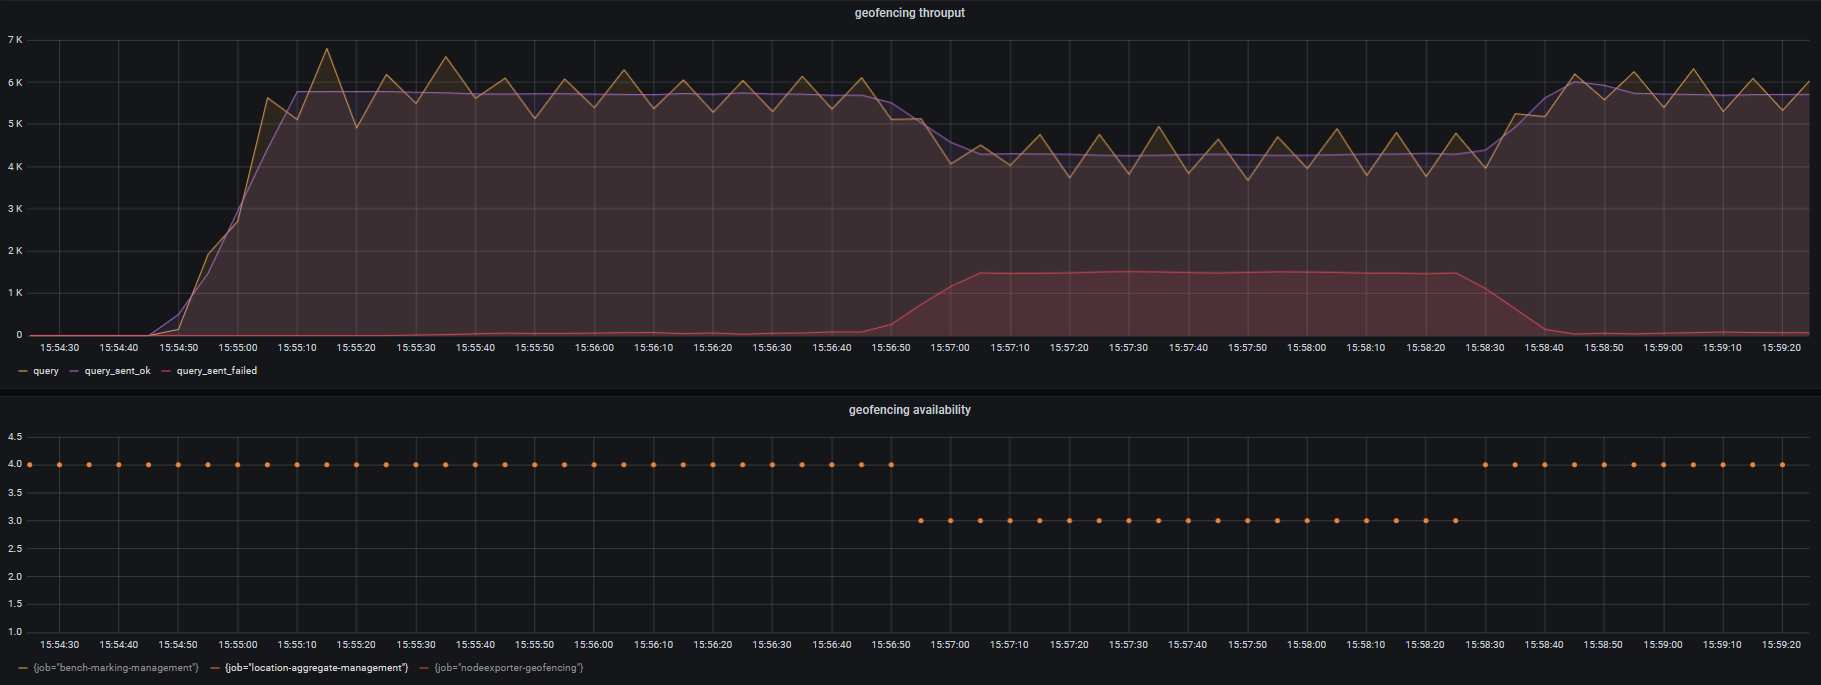
\includegraphics[width=\linewidth, scale=2]{images/evaluation/ex7-benchmarking-ongoing-2per10sec.png}
    \end{figure}

    In figure \ref{fig:ex7} the purple line is the input rate (number of queries received by FenceX per
    second) and the yellow line shows the rate of queries answered successfully.
    Red line shows how many queries FenceX failed to respond.
    A failure to respond in this load range means that the service supposed to answer the query was not
    up and running at that moment.
    It is clear that once one of the instances of poll leg goes because of restart, the throughput drops and error
    rate goes up accordingly.
    Once restart and re-balancing finishes successfully, the throughput increases back to the previous
    value and error rate drops back to zero.
    Please note that re-balancing has no direct affect on queries by fence.
    However, health of each Kafka or Kafka Stream application is dependent on a successful re-balancing.

    \subsubsection{Conclusion of poll leg availability evaluation}
    Poll leg of FenceX can handle some of it's instances going down and coming back up.
    Even if an unhealthy instance does not recover, the only effect will be on the overall throughput of system
    temporarily.


    \section{Strong scalability}
    If a software has strong scalability properties means providing same load, the more you scale it out, the better
    it performs.
    For a given circumstance, there might be a point after which scaling out more won't affect the performance anymore.
    The load can be data set size, table size or incoming HTTP query rate.
    Performance is also case and context dependent.
    It can be query latency or throughput.
    In stream processing systems the load is the rate of input, rate of incoming events, the rate at which source
    produces input in to the pipeline.
    In FenceX, for poll leg, similar to previous experiments, load is rate of incoming HTTP requests for queries by fence.
    And, for push leg is the rate at which location reports arrive.
    Performance in our experiments is throughput of push leg and poll leg.
    We expeect FenceX to show strong scalability characteristics in both of its legs.

    \subsection{Push leg}
    Push leg strong scalability evaluation scenario:
    \begin{itemize}
        \item[1-] Define fences for movers using all the trips in the bench-marking application database.
        \item[2-] Start an ongoing stream of location reports with fixed rate toward FenceX.
        \item[3-] Deploy only one instance of realtime-fencing (should not to be rich in resources as we want it to
        be overwhelmed).
        \item[4-] Check the throughput.
        Hopefully it is much lower than the input rate.
        \item[5-] Deploy one more instances of realtime-fencing with exactly same resources as previous one.
        \item[6-] Assert an increase in throughput.
        \item[7-] Keep adding instances and asserting increase in throughput until throughput stops increasing.
    \end{itemize}

    During these experiments, each time we deploy one more instance of realtime-fencing, a re-balancing happens which
    avoids some incoming location updates from being processed.
    Those location updates get buffered in the topic and after re-balancing will get their chance to be processed.
    A direct consequence of such buffering is that at some points in the experiments, the throughput we observe is
    higher than the input rate.
    This is because the input stream is ongoing and fixed rate, so process of buffered location updates only adds to
    throughput in that specific moments.

    \clearpage

    \subsubsection{Experiment 8}
    \begin{table}[h!]
        \centering
        \begin{tabular}{|c|c|c|c|}
            \hline
            Application               & number of instances & CPU(MHz) & RAM(MB) \\
            \hline
            location-update-publisher & 4                   & 200      & 700     \\
            location-aggregate        & -                   & -        & -       \\
            realtime-fencing          & 1                   & 30       & 500     \\
            \hline
        \end{tabular}
        \caption{Experiment 8 deployment view}
        \label{table:ex8-dv}
    \end{table}

    Table \ref{table:ex8-dv} shows, for experiment 8, how many instances of each FenceX microservices we have initially
    deployed in addition to the amount of resources we have assigned to each.
    The row in table \ref{table:ex8-dv} with no values corresponds to a microservice which does not relate to the
    experiment 8.
    The following figure illustrates how input rate and throughput have changed during experiment 8.
    It also shows number of deployed instances of related microservices during this experiment.

    \begin{figure}[h!]
        \centering
        \caption{FenceX push leg strong scalability ex8}
        \label{fig:ex8}
        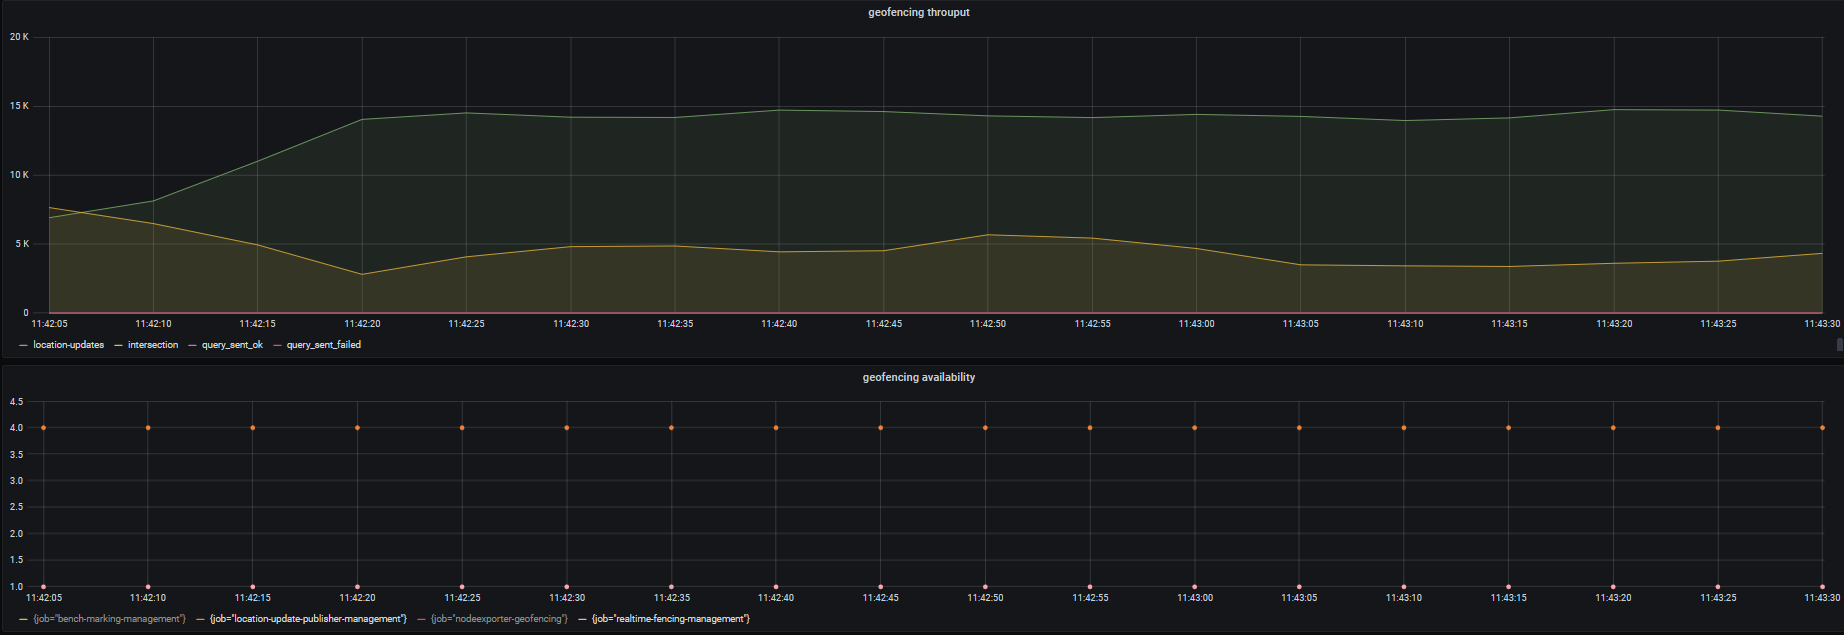
\includegraphics[width=\linewidth, scale=2]{images/evaluation/ex8-benchmarking-ongoing-2per4sec.png}
    \end{figure}

    In figure \ref{fig:ex8} the green line is essentially the input rate (number of location updates per second),
    yellow line represents throughput (number of fence point intersections) and the pink dots shows number of
    deployed instances of realtime-fencing.
    Figures in following push leg strong scalability experiments can also be read in the same way.

    So figure \ref{fig:ex8} illustrates that one instance of realtime-fencing with the rather low given resources, can
    only handle one 3rd of input rate.
    Which is 5k intersections per second out of 15k location updates per second.

    \clearpage

    \subsubsection{Experiment 9}
    \begin{table}[h!]
        \centering
        \begin{tabular}{|c|c|c|c|}
            \hline
            Application               & number of instances & CPU(MHz) & RAM(MB) \\
            \hline
            location-update-publisher & 4                   & 200      & 700     \\
            location-aggregate        & -                   & -        & -       \\
            realtime-fencing          & 2                   & 30       & 500     \\
            \hline
        \end{tabular}
        \caption{Experiment 9 deployment view}
        \label{table:ex9-dv}
    \end{table}

    Table \ref{table:ex9-dv} shows, for experiment 9, how many instances of each FenceX microservices we have
    deployed in addition to the amount of resources we have assigned to each.
    Compared to experiment 8, we have deployed one more instance of realtime-fencing.
    The row in table \ref{table:ex9-dv} with no values corresponds to a microservice which does not relate to the
    experiment 9.
    The following figure illustrates how input rate and throughput have changed during experiment 9.
    It also shows how (and when) number of deployed instances of related microservices has changed during this
    experiment.

    \begin{figure}[h!]
        \centering
        \caption{FenceX push leg strong scalability ex9}
        \label{fig:ex9}
        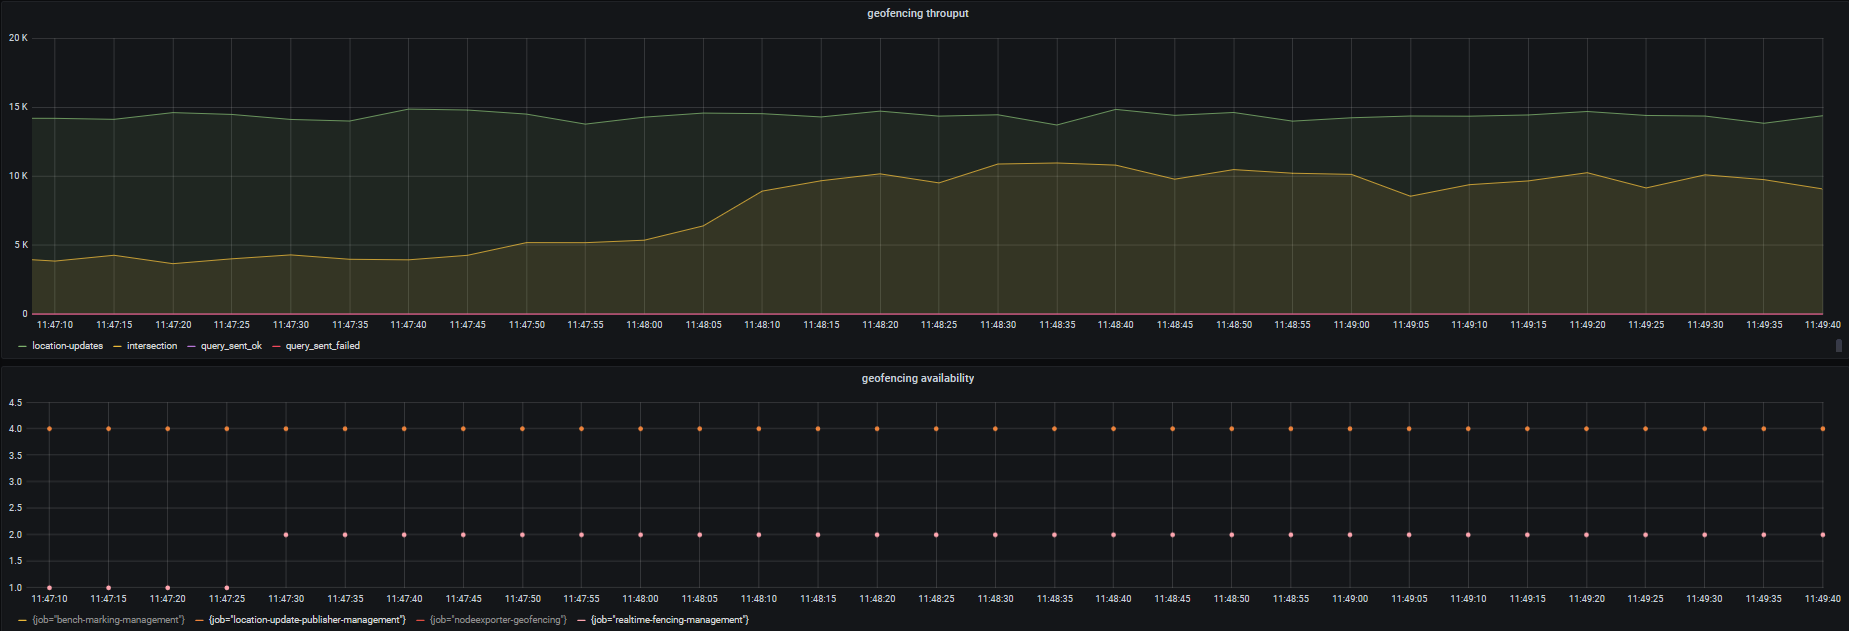
\includegraphics[width=\linewidth, scale=2]{images/evaluation/ex9-benchmarking-ongoing-2per4sec.png}
    \end{figure}

    Looking at figure \ref{fig:ex9} we can easily observe that once the second instance is up and running, after
    re-balancing, throughput goes proportionally up, from 5k/s to 10k/s.
    At this point we can guess that without changing anything, just adding one more instance of realtime-fencing
    should be enough to cover the whole 15k/s input rate.
    15K location updates per second is the highest input rate that we could produce in a stable manner.

    \clearpage

    \subsubsection{Experiment 10}
    \begin{table}[h!]
        \centering
        \begin{tabular}{|c|c|c|c|}
            \hline
            Application               & number of instances & CPU(MHz) & RAM(MB) \\
            \hline
            location-update-publisher & 4                   & 200      & 700     \\
            location-aggregate        & -                   & -        & -       \\
            realtime-fencing          & 3                   & 30       & 500     \\
            \hline
        \end{tabular}
        \caption{Experiment 10 deployment view}
        \label{table:ex10-dv}
    \end{table}

    Table \ref{table:ex10-dv} shows, for experiment 10, how many instances of each FenceX microservices we have
    deployed in addition to the amount of resources we have assigned to each.
    Compared to experiment 9, we have deployed one more instance of realtime-fencing.
    The row in table \ref{table:ex10-dv} with no values corresponds to a microservice which does not relate to the
    experiment 10.
    The following figure illustrates how input rate and throughput have changed during experiment 10.
    It also shows how (and when) number of deployed instances of related microservices has changed during this
    experiment.

    \begin{figure}[h!]
        \centering
        \caption{FenceX push leg strong scalability ex10}
        \label{fig:ex10}
        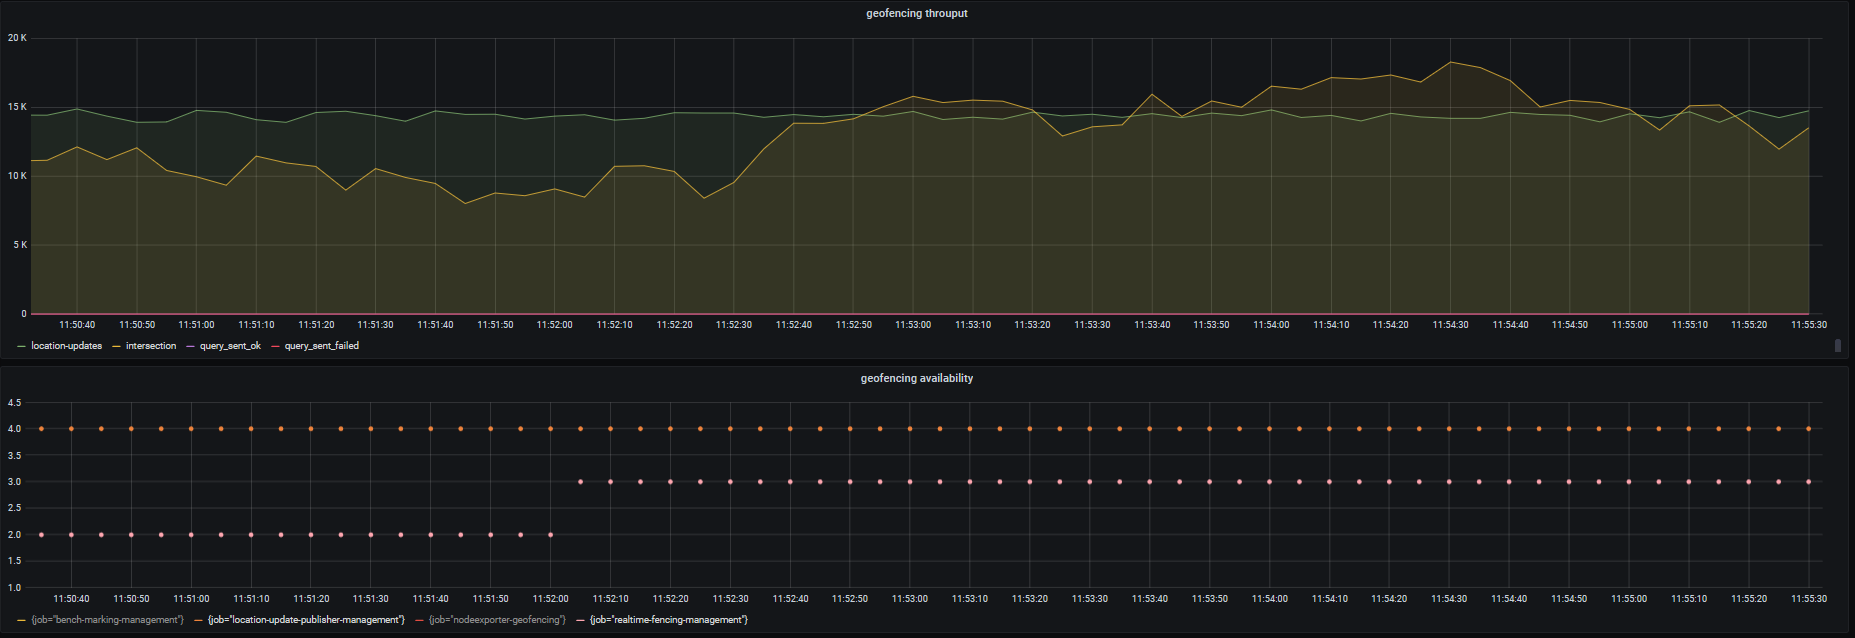
\includegraphics[width=\linewidth, scale=2]{images/evaluation/ex10-benchmarking-ongoing-2per4sec.png}
    \end{figure}

    As we expected, deploying three instances of realtime-fencing with the given resources, was enough to process 15K
    location updates per second.
    Also in \ref{fig:ex10} we can see effect of buffered location updates on throughput.
    Around the end parts of the graph, throughput is higher than input rate.

    \clearpage

    \subsubsection{Experiment 11}
    Now in order to be just sure that adding more instances, won't affect the throughput in any good or bad way, we
    add another instance as the final step.

    \begin{table}[h!]
        \centering
        \begin{tabular}{|c|c|c|c|}
            \hline
            Application               & number of instances & CPU(MHz) & RAM(MB) \\
            \hline
            location-update-publisher & 4                   & 200      & 700     \\
            location-aggregate        & -                   & -        & -       \\
            realtime-fencing          & 4                   & 30       & 500     \\
            \hline
        \end{tabular}
        \caption{Experiment 11 deployment view}
        \label{table:ex11-dv}
    \end{table}

    Table \ref{table:ex11-dv} shows, for experiment 11, how many instances of each FenceX microservices we have
    deployed in addition to the amount of resources we have assigned to each.
    Compared to experiment 10, we have deployed one more instance of realtime-fencing.
    The row in table \ref{table:ex11-dv} with no values corresponds to a microservice which does not relate to the
    experiment 11.
    The following figure illustrates how input rate and throughput have changed during experiment 11.
    It also shows how (and when) number of deployed instances of related microservices has changed during this
    experiment.

    \begin{figure}[h!]
        \centering
        \caption{FenceX push leg strong scalability ex11}
        \label{fig:ex11}
        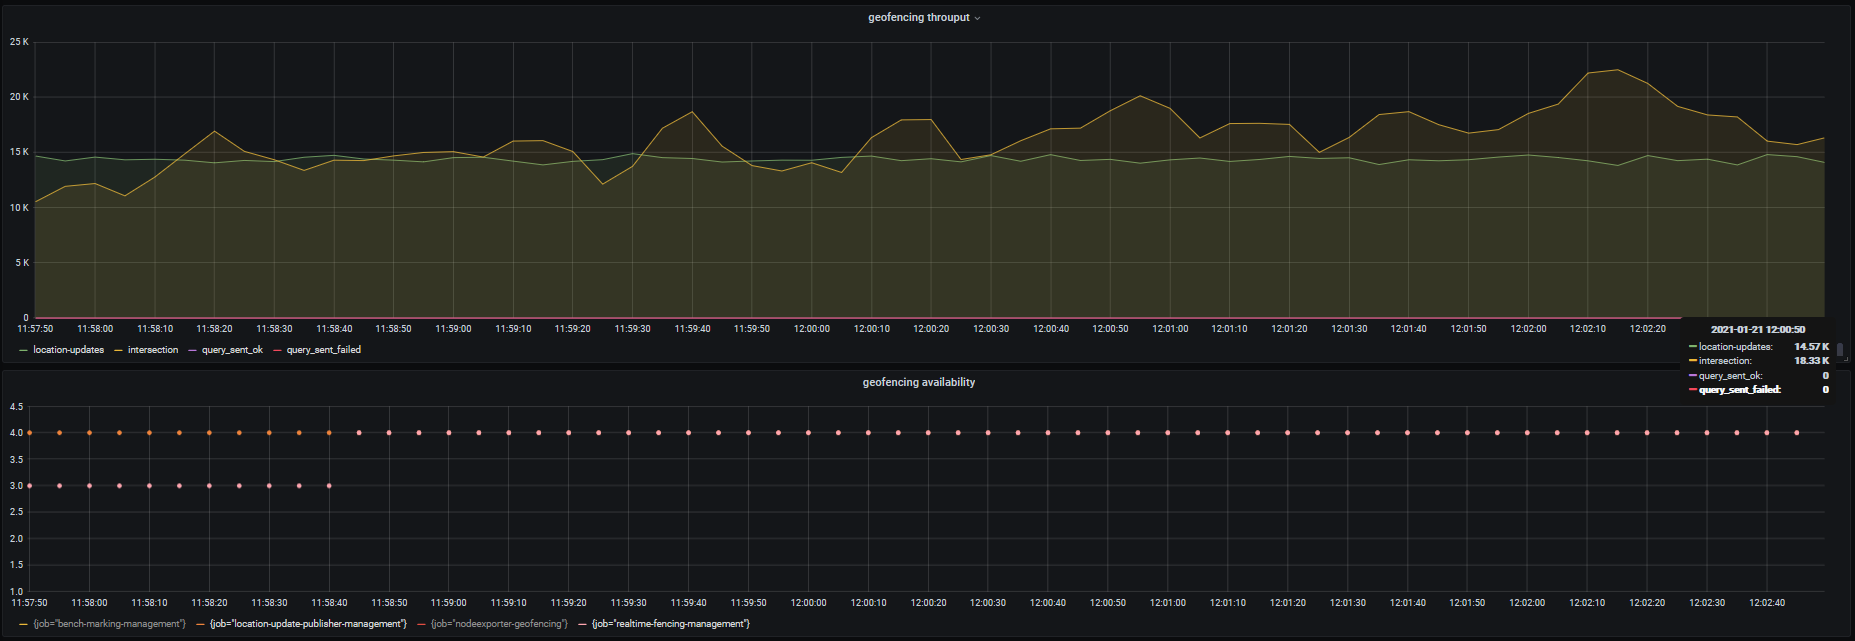
\includegraphics[width=\linewidth, scale=2]{images/evaluation/ex11-benchmarking-ongoing-2per4sec.png}
    \end{figure}

    The clear observation is that adding one more instance didn't have any special effect on the throughput.
    This is expected since throughput can not exceed input rate regardless of processing power.
    However, we can again see the effect of buffered location updates during re-balancing pretty much all over the
    graph.

    \subsubsection{Conclusion of push leg strong scalability evaluation}
    Push leg of FenceX has strong scalability characteristics at least in the range of input rate we have managed to produce.
    So in case of unexpectedly high load, just scaling realtime-fencing out can prove effective.

    \subsection{Poll leg}
    Poll leg strong scalability evaluation scenario:
    \begin{itemize}
        \item[1-] Send location reports for movers using all the trips in the bench-marking application database.
        \item[2-] Start an ongoing load of queries (query by fence) with fixed rate.
        \item[3-] Deploy only one instance of location-aggregate (should not be too rich in resources, we want it to be
        overwhelmed).
        \item[4-] Check the throughput. Hopefully it is much lower than the input rate.
        \item[5-] Deploy one more instances of location-aggregate with exactly same resources as previous one.
        \item[6-] Assert an increase in throughput.
        \item[7-] Keep adding instances and asserting increase in throughput until throughput stops increasing.
    \end{itemize}

    During these experiments, each time we deploy one more instance of location-aggregate, a re-balancing happens which
    avoids some queries from being answered.
    Those queries will be considered as failed.

    \clearpage

    \subsubsection{Experiment 17}
    \begin{table}[h!]
        \centering
        \begin{tabular}{|c|c|c|c|}
            \hline
            Application               & number of instances & CPU(MHz) & RAM(MB) \\
            \hline
            location-update-publisher & 1                   & 200      & 700     \\
            location-aggregate        & 1                   & 100      & 1500    \\
            realtime-fencing          & -                   & -        & -       \\
            \hline
        \end{tabular}
        \caption{Experiment 17 deployment view}
        \label{table:ex17-dv}
    \end{table}

    Table \ref{table:ex17-dv} shows, for experiment 17, how many instances of each FenceX microservices we have
    initially deployed in addition to the amount of resources we have assigned to each.
    The row in table \ref{table:ex17-dv} with no values corresponds to a microservice which does not relate to the
    experiment 17.
    The following figure illustrates how input rate and throughput have changed during experiment 17.
    It also shows how many instances of related microservices were up and running during this experiment.

    \begin{figure}[h!]
        \centering
        \caption{FenceX poll leg strong scalability ex17}
        \label{fig:ex17}
        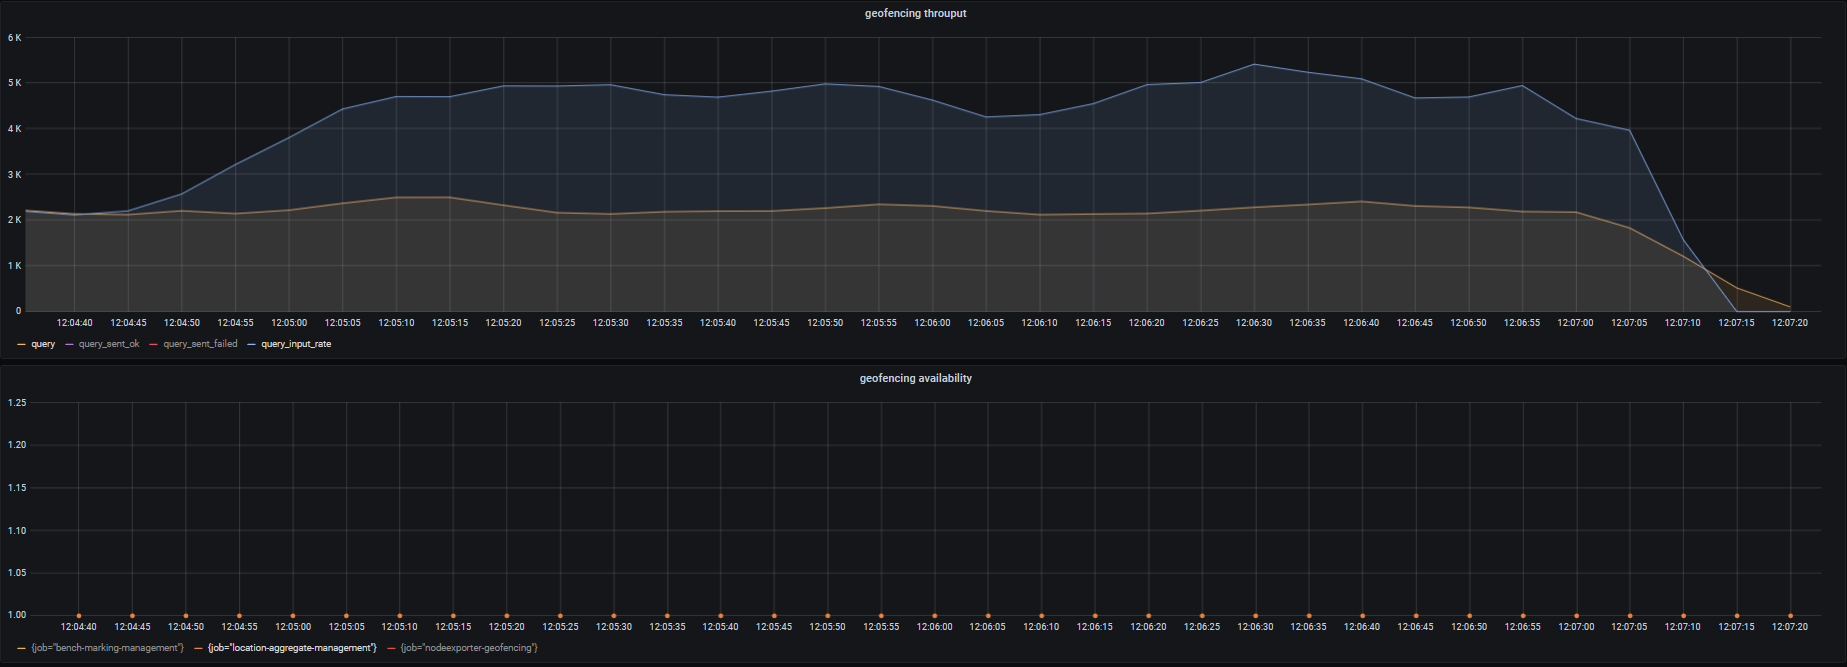
\includegraphics[width=\linewidth, scale=2]{images/evaluation/ex17-benchmarking-ongoing-2per4sec.png}
    \end{figure}

    \clearpage

    \subsubsection{Experiment 18}
    \begin{table}[h!]
        \centering
        \begin{tabular}{|c|c|c|c|}
            \hline
            Application               & number of instances & CPU(MHz) & RAM(MB) \\
            \hline
            location-update-publisher & 0                   & -        & -       \\
            location-aggregate        & 2                   & 100      & 1500    \\
            realtime-fencing          & -                   & -        & -       \\
            \hline
        \end{tabular}
        \caption{Experiment 18 deployment view}
        \label{table:ex18-dv}
    \end{table}

    Table \ref{table:ex18-dv} shows, for experiment 18, how many instances of each FenceX microservices we have
    deployed in addition to the amount of resources we have assigned to each.
    Compared to experiment 17, we have deployed one more instance of location-aggregate.
    The row in table \ref{table:ex18-dv} with no values corresponds to a microservice which does not relate to the
    experiment 18.
    The following figure illustrates how input rate and throughput have changed during experiment 18.
    It also shows how many instances of related microservices were up and running during this experiment.

    \begin{figure}[h!]
        \centering
        \caption{FenceX poll leg strong scalability ex18}
        \label{fig:ex18}
        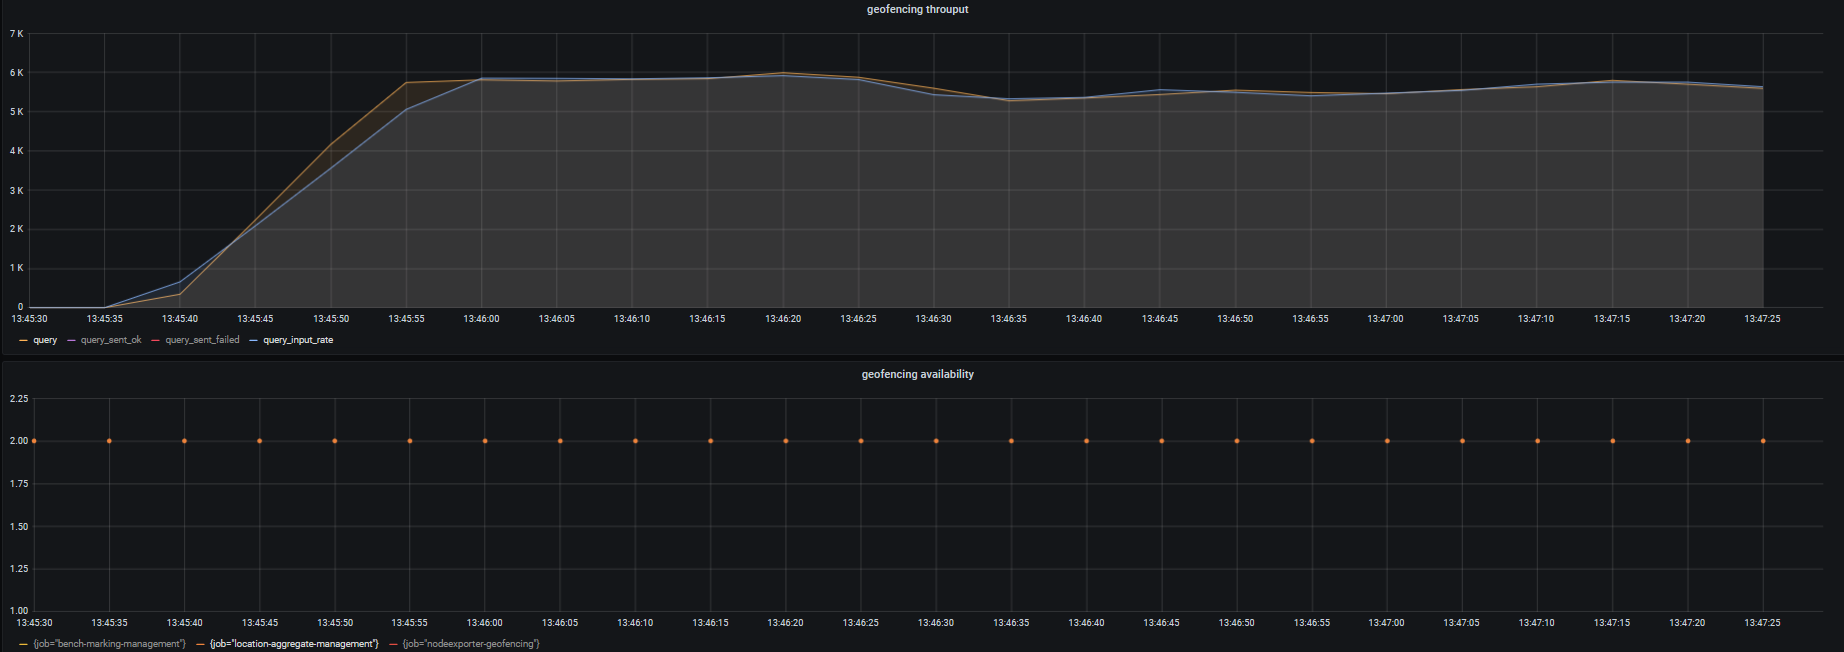
\includegraphics[width=\linewidth, scale=2]{images/evaluation/ex18-benchmarking-ongoing-2per4sec.png}
    \end{figure}

    In figures \ref{fig:ex17} and \ref{fig:ex18} the blue line represents input rate, number of incoming HTTP
    requests.
    Orange line illustrates throughput which is number of queries responded successfully.
    Orange dots, show how many instances of location-aggregate are up and running.
    As figures show, FenceX has managed to handle 2k queries per second with one not so rich instance of location-aggregate.
    Adding one more instance resulted in throughput becoming equal to input rate (~6K queries per second).

    One of the differences between push and poll leg is that the minimum resources required for poll leg to function
    smoothly is much higher than push leg.
    This is due to the fact that poll leg has global in memory data store.
    Also, the amount of data exists in poll leg is substantially higher.
    There is usually way more location updates for each mover than fences.
    In fact currently, there will be at most one fence in push leg for each mover compared to many location updates
    in poll leg.

    As an overall consequence, when we deploy even one instance of location-aggregate, it's already rich enough to be
    able to answer many HTTP requests (query by fence).
    Which is about half of the input rate we can produce at maximum in a stable ongoing manner.
    So when we deploy two instances of location-aggregate with the mentioned resources, two available instances just
    handle our full capacity of input load production.
    So there is no point in continuing strong scalability experiments for poll leg withing this range of input.

    \subsubsection{Conclusion of poll leg strong scalability evaluation}
    Poll leg of FenceX has strong scalability characteristics at least in the range of input rate we have managed to
    produce.
    So in case of unexpectedly high load, just scaling realtime-fencing out can prove effective.


    \section{Weak scalability}
    If a software has weak scalability properties, it means providing a load which is increasing step by step over
    time, the more you scale the software out, the better it performs.
    For a given circumstance, there might be a point after which more scale out or more load won't affect
    the performance anymore.
    The load can be data set size, table size or incoming HTTP query rate.
    Performance is also case and context dependent.
    It can be query latency or throughput.
    In stream processing systems, load is the rate of input, rate of incoming events, the rate at
    which source publishes input in to the pipeline.
    In FenceX, for poll leg, similar to previous experiments, load is rate of incoming HTTP requests for queries by
    fence.
    And, for push leg is the rate at which location reports arrive.
    Performance in case of our experiments, is throughput of push leg and poll leg.
    We expect both legs of FenceX to have weak scalability characteristic.

    \subsection{Push leg}
    Push leg weak scalability evaluation scenario:
    \begin{itemize}
        \item[1-] Define fences for movers using all the trips in the bench-marking application database.
        \item[2-] Start an ongoing stream of location reports with fixed low rate toward FenceX.
        \item[3-] Deploy only one instance of realtime-fencing (should not be too rich in resources as we want it to
        be overwhelmed).
        \item[4-] Check the throughput. Hopefully it is equal to input rate.
        \item[5-] Deploy one more instances of realtime-fencing with exactly same resources as previous one. Also,
        increase the input rate (like double).
        \item[6-] Assert that throughput covers the input rate.
        \item[7-] Keep adding instances, increasing input rate and asserting increase in throughput until throughput
        stops increasing.
    \end{itemize}

    During these experiments, each time we deploy one more instance of realtime-fencing, a re-balancing happens which
    avoids some incoming location updates from being processed.
    Those location updates get buffered in the topic and after re-balancing will get their chance to be processed.
    A direct consequence of such buffering is that at some points in the experiments, the throughput we observe might be
    higher than the input rate.
    This is because the input stream is ongoing and fixed rate.

    \clearpage

    \subsubsection{Experiment 19}
    \begin{table}[h!]
        \centering
        \begin{tabular}{|c|c|c|c|}
            \hline
            Application               & number of instances & CPU(MHz) & RAM(MB) \\
            \hline
            location-update-publisher & 4                   & 400      & 700     \\
            location-aggregate        & -                   & -        & -       \\
            realtime-fencing          & 1                   & 60       & 500     \\
            \hline
        \end{tabular}
        \caption{Experiment 19 deployment view}
        \label{table:ex19-dv}
    \end{table}

    Table \ref{table:ex19-dv} shows, for experiment 19, how many instances of each FenceX microservices we have
    initially deployed in addition to the amount of resources we have assigned to each.
    The row in table \ref{table:ex19-dv} with no values corresponds to a microservice which does not relate to the
    experiment 19.
    The following figure illustrates how input rate and throughput have changed during experiment 19.
    It also shows how many instances of related microservices were up and running during this experiment.

    \begin{figure}[h!]
        \centering
        \caption{FenceX push leg weak scalability ex19}
        \label{fig:ex19}
        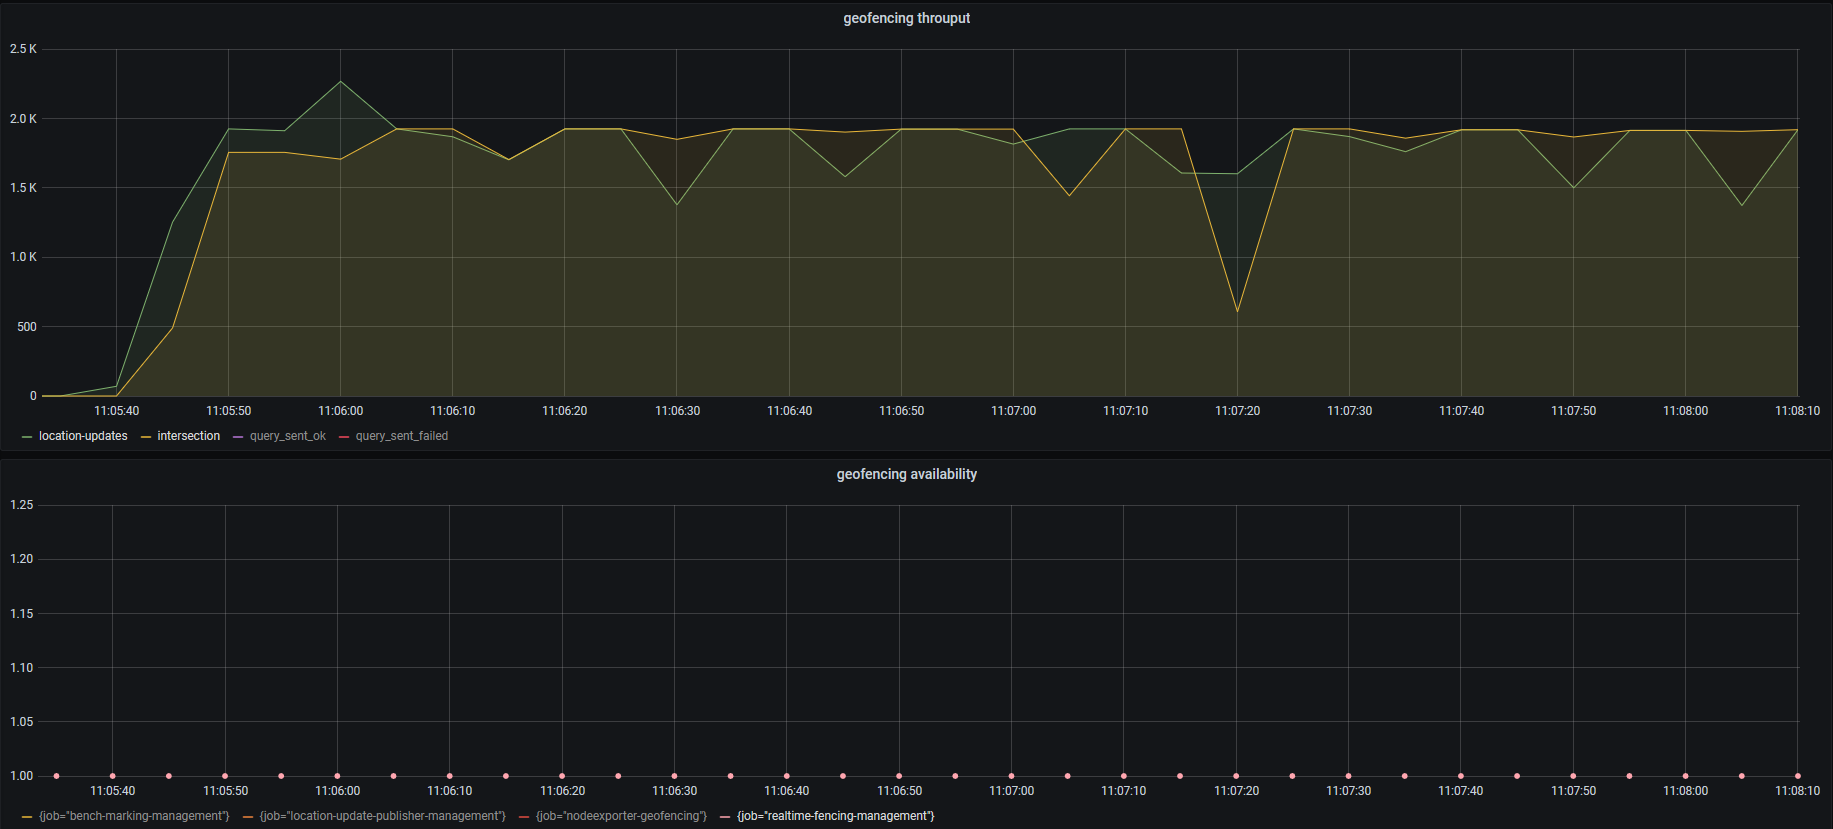
\includegraphics[width=\linewidth, scale=2]{images/evaluation/ex19-benchmarking-ongoing-1per16sec.png}
    \end{figure}

    In figure \ref{fig:ex19} the green line is input rate (number of location updates per second),
    yellow line represents throughput (number of fence point intersections) and the pink dots shows number of
    deployed instances of realtime-fencing.
    Figures in following push leg weak scalability experiments can also be read in the same way as experiment 19.

    So far with one limited in resources instance of realtime-fencing, FenceX has managed to deal with around 2K
    location updates per second successfully in a stable manner.

    \clearpage

    \subsubsection{Experiment 20}
    \begin{table}[h!]
        \centering
        \begin{tabular}{|c|c|c|c|}
            \hline
            Application               & number of instances & CPU(MHz) & RAM(MB) \\
            \hline
            location-update-publisher & 4                   & 400      & 700     \\
            location-aggregate        & -                   & -        & -       \\
            realtime-fencing          & 2                   & 60       & 500     \\
            \hline
        \end{tabular}
        \caption{Experiment 20 deployment view}
        \label{table:ex20-dv}
    \end{table}

    Table \ref{table:ex20-dv} shows, for experiment 20, how many instances of each FenceX microservices we have
    deployed in addition to the amount of resources we have assigned to each.
    Compared to experiment 19, we have deployed one more instance of realtime-fencing.
    The row in table \ref{table:ex20-dv} with no values corresponds to a microservice which does not relate to the
    experiment 20.
    The following figure illustrates how input rate and throughput have changed during experiment 20.
    It also shows how many instances of related microservices were up and running during this experiment.

    \begin{figure}[h!]
        \centering
        \caption{FenceX push leg weak scalability ex20}
        \label{fig:ex20}
        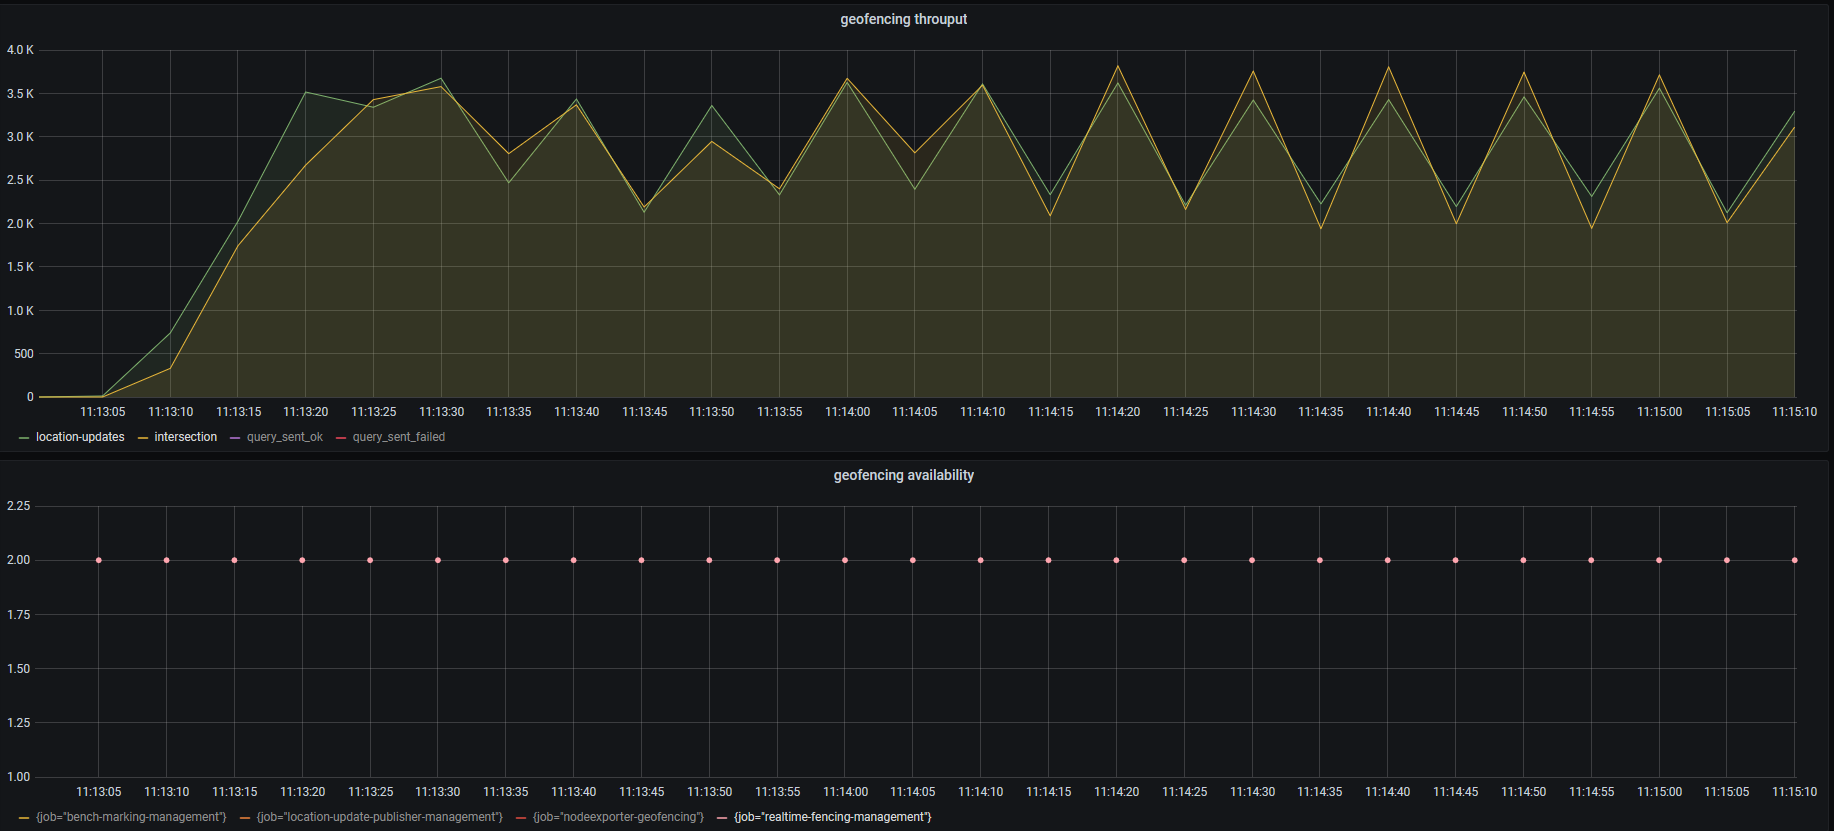
\includegraphics[width=\linewidth, scale=2]{images/evaluation/ex20-benchmarking-ongoing-1per10sec.png}
    \end{figure}

    Two such instances of realtime-fencing managed to handle around 3K location updates per second.

    \clearpage

    \subsubsection{Experiment 21}
    \begin{table}[h!]
        \centering
        \begin{tabular}{|c|c|c|c|}
            \hline
            Application               & number of instances & CPU(MHz) & RAM(MB) \\
            \hline
            location-update-publisher & 4                   & 400      & 700     \\
            location-aggregate        & -                   & -        & -       \\
            realtime-fencing          & 4                   & 60       & 500     \\
            \hline
        \end{tabular}
        \caption{Experiment 21 deployment view}
        \label{table:ex21-dv}
    \end{table}

    Table \ref{table:ex21-dv} shows, for experiment 21, how many instances of each FenceX microservices we have
    deployed in addition to the amount of resources we have assigned to each.
    Compared to experiment 20, we have deployed one more instance of realtime-fencing.
    The row in table \ref{table:ex21-dv} with no values corresponds to a microservice which does not relate to the
    experiment 21.
    The following figure illustrates how input rate and throughput have changed during experiment 21.
    It also shows how many instances of related microservices were up and running during this experiment.

    \begin{figure}[h!]
        \centering
        \caption{FenceX push leg weak scalability ex21}
        \label{fig:ex21}
        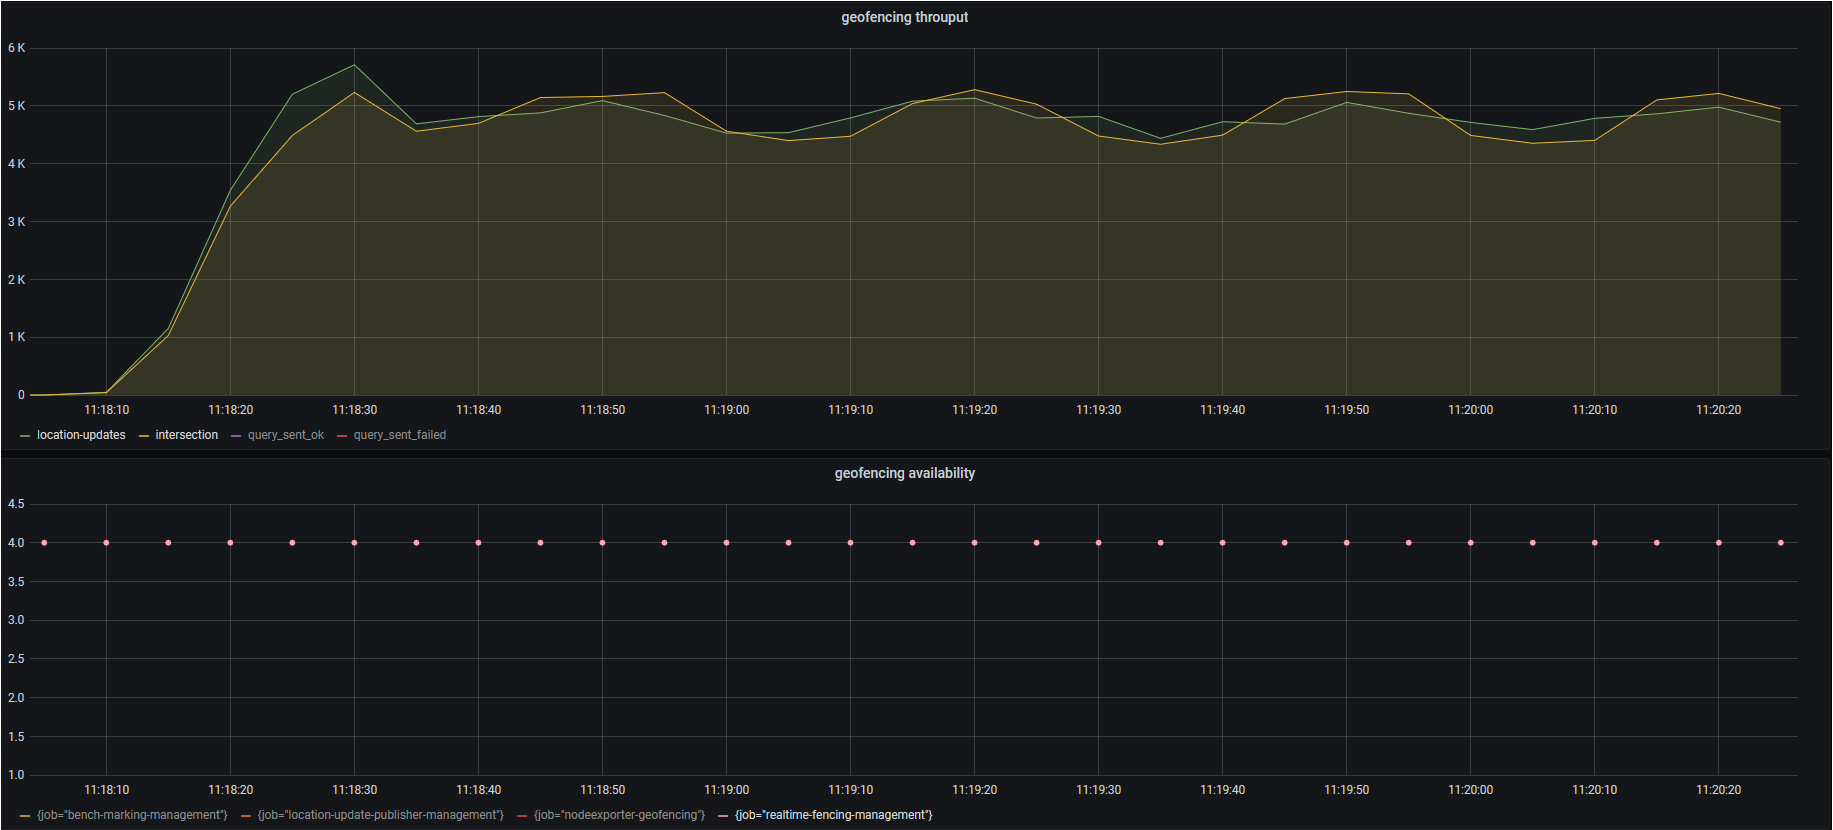
\includegraphics[width=\linewidth, scale=2]{images/evaluation/ex21-benchmarking-ongoing-1per6sec.png}
    \end{figure}
    Four such instances of realtime-fencing managed to handle around 5K location updates per second.

    \clearpage

    \subsubsection{Experiment 22}
    \begin{table}[h!]
        \centering
        \begin{tabular}{|c|c|c|c|}
            \hline
            Application               & number of instances & CPU(MHz) & RAM(MB) \\
            \hline
            location-update-publisher & 4                   & 400      & 700     \\
            location-aggregate        & -                   & -        & -       \\
            realtime-fencing          & 5                   & 60       & 500     \\
            \hline
        \end{tabular}
        \caption{Experiment 22 deployment view}
        \label{table:ex22-dv}
    \end{table}

    Table \ref{table:ex22-dv} shows, for experiment 22, how many instances of each FenceX microservices we have
    deployed in addition to the amount of resources we have assigned to each.
    Compared to experiment 21, we have deployed one more instance of realtime-fencing.
    The row in table \ref{table:ex22-dv} with no values corresponds to a microservice which does not relate to the
    experiment 22.
    The following figure illustrates how input rate and throughput have changed during experiment 22.
    It also shows how many instances of related microservices were up and running during this experiment.

    \begin{figure}[h!]
        \centering
        \caption{FenceX push leg weak scalability ex22}
        \label{fig:ex22}
        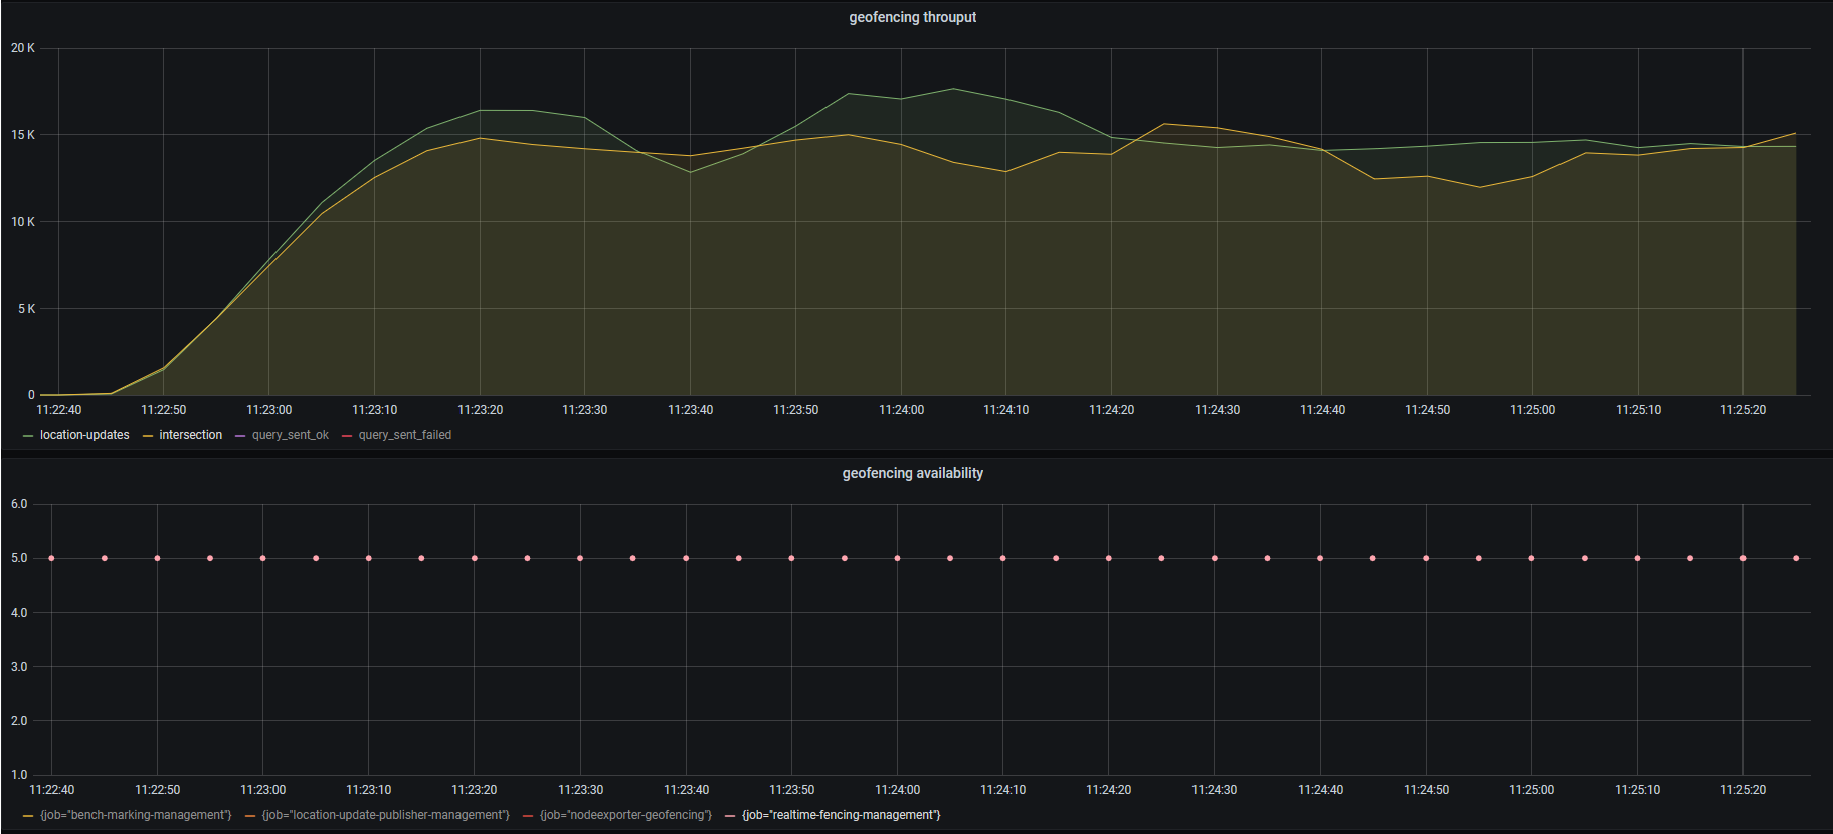
\includegraphics[width=\linewidth, scale=2]{images/evaluation/ex22-benchmarking-ongoing-1per2sec.png}
    \end{figure}
    Five instances of realtime-fencing managed to handle around 15K location updates per second.

    \clearpage

    \subsubsection{Experiment 23}
    \begin{table}[h!]
        \centering
        \begin{tabular}{|c|c|c|c|}
            \hline
            Application               & number of instances & CPU(MHz) & RAM(MB) \\
            \hline
            location-update-publisher & 4                   & 400      & 700     \\
            location-aggregate        & -                   & -        & -       \\
            realtime-fencing          & 10                  & 60       & 500     \\
            \hline
        \end{tabular}
        \caption{Experiment 23 deployment view}
        \label{table:ex23-dv}
    \end{table}

    Table \ref{table:ex23-dv} shows, for experiment 23, how many instances of each FenceX microservices we have
    deployed in addition to the amount of resources we have assigned to each.
    Compared to experiment 22, we have deployed one more instance of realtime-fencing.
    The row in table \ref{table:ex23-dv} with no values corresponds to a microservice which does not relate to the
    experiment 23.
    The following figure illustrates how input rate and throughput have changed during experiment 23.
    It also shows how many instances of related microservices were up and running during this experiment.

    \begin{figure}[h!]
        \centering
        \caption{FenceX push leg weak scalability ex23}
        \label{fig:ex23}
        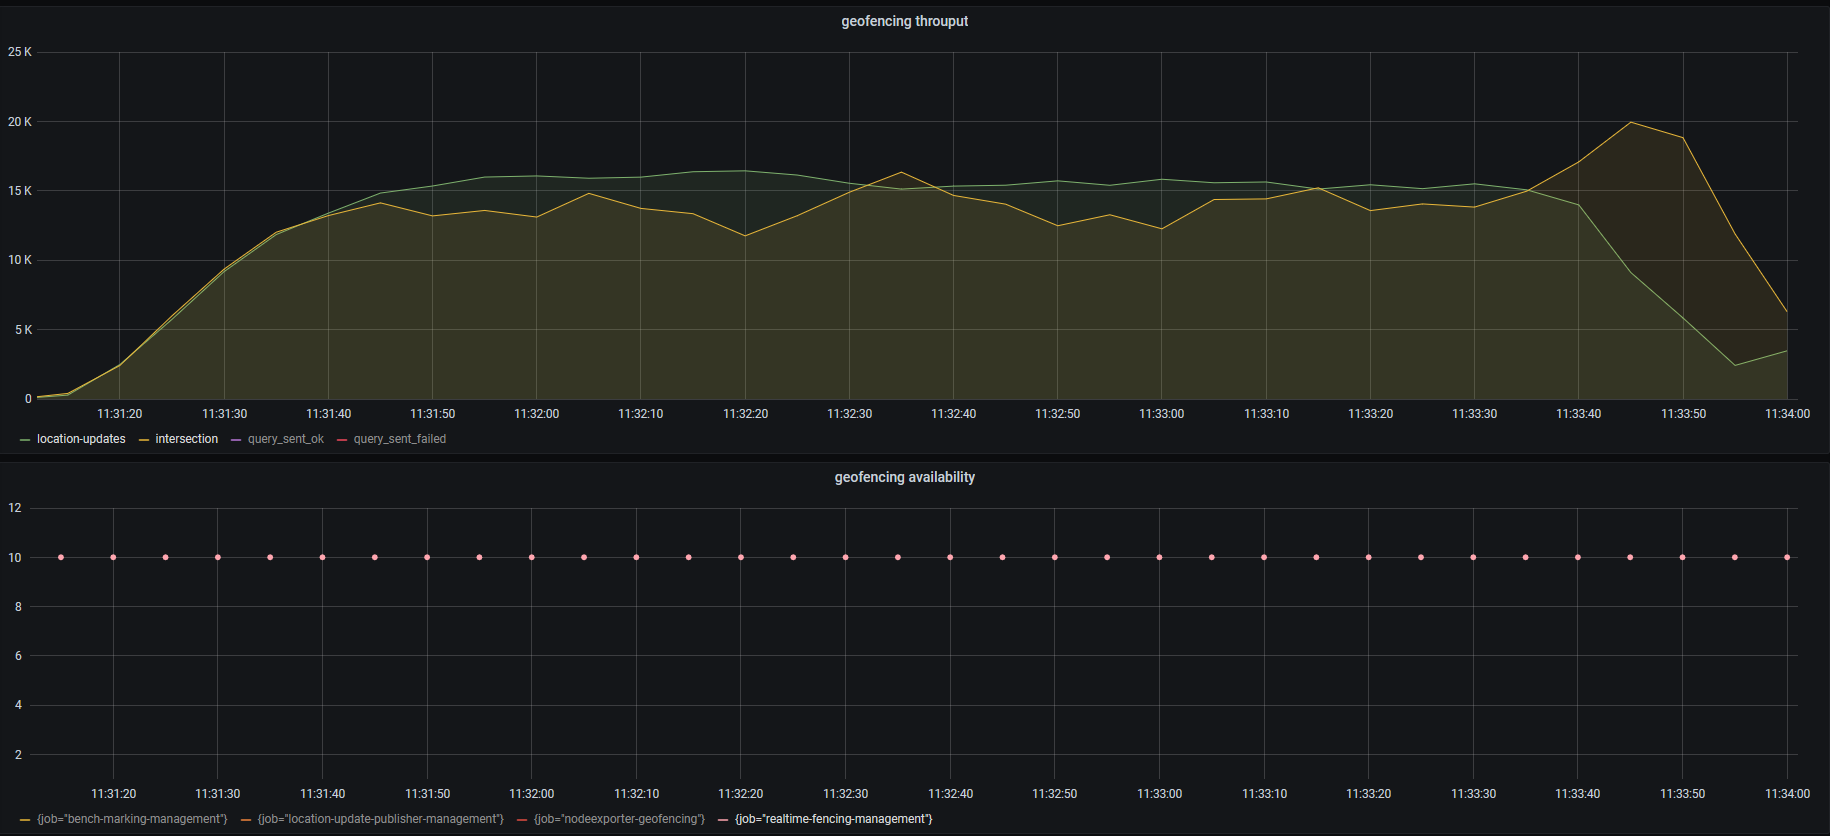
\includegraphics[width=\linewidth, scale=2]{images/evaluation/ex23-benchmarking-ongoing-2per2sec.png}
    \end{figure}

    Ten such instances of realtime-fencing managed to handle around 15K location updates per second.
    However, in experiment 23 our intention was to increase input rate to above 15k/s which we did not manage due to
    limitations on the available resources to bench-marking application.
    So we will not continue weak scalability experiments for push log further.

    \subsubsection{Conclusion of push leg weak scalability evaluation}
    We observed that as we increased input rate and deployed more instances of push leg of FenceX, push leg
    throughput got higher.
    So push leg of FenceX managed to scale well in face of increasing load and it has weak scalability characteristics.

    \subsection{Poll leg}
    Poll leg weak scalability evaluation scenario:
    \begin{itemize}
        \item[1-] Send location updates for movers using all the trips in the bench-marking application database.
        \item[2-] Start an ongoing load of queries (query by fence) with fixed low rate.
        \item[3-] Deploy only one instance of location-aggregate (should not be too rich in resources, we want it to
        be overwhelmed).
        \item[4-] Check the throughput. Hopefully it is equal to input rate.
        \item[5-] Deploy one more instances of location-aggregate with exactly same resources as previous one. Also,
        increase the input rate (like double).
        \item[6-] Assert that throughput covers the input rate.
        \item[7-] Keep adding instances, increasing input rate and asserting increase in throughput until throughput
        stops increasing.
    \end{itemize}

    Relaying on the observations from previous experiments, two instances of location-aggregate (with minimum
    resources for working smoothly) can easily cover our maximum capacity for producing input load.
    So there is no point in carrying out weak scalability experiments for poll leg.


    \section{Free fall scalability}
    In order to stress test stream processing systems or when trying to find out how they can scale under high rates
    of input load, naturally we need to be able to produce high rates of input in the first place.
    This can be challenging when the input data is complex to produce and/or available resources to our input
    producers is limited.
    Stream processing systems relay on some sort of buffering which means events should be stored somewhere so
    that processors can handle them when they are ready.
    That's how they get some sort of back pressure in reactive systems terminology.
    In case of FenceX, that buffer is the Kafka topics which can grow very large without any problem.

    So instead of trying to produce a high rate of input in realtime, we can buffer large number of events in a Kafka
    topic (waiting to be picked up and processed) while processors are down.
    When enough events got accumulated, we stop buffering event and deploy event processors.
    Now processors can read the events with the least possible IO involved.
    Applying this approach, we can assess how well an event processor can be scaled when there is almost no factor
    involved other than input rate and processing power.

    This style of testing is only applicable to push leg since the concept of buffering work differently in terms of
    HTTP request.
    Basically HTTP based communication does not support back pressure.

    \subsection{Push leg}
    Push leg free fall scalability evaluation scenario:
    \begin{itemize}
        \item[1-] Play with different input rates and deployment configurations to get a feeling of how to tune the
        system for best performance
        \item[2-] Undeploy all realtime-fencing instances.
        \item[3-] Start an ongoing stream of location reports with fixed rate toward FenceX.
        \item[4-] Wait 5 minutes or so.
        \item[5-] Now that there is plenty of location updates buffered in the Kafka topic, stop the stream of
        location updates.
        \item[6-] Deploy realtime-fencing instances according to the previously discovered deployment configuration.
        \item[7-] Check the throughput and assert that it's much higher than maxixmum oberserved throughput in
        previous experiments.
    \end{itemize}

    \subsubsection{Experiment 24}
    \begin{table}[h!]
        \centering
        \begin{tabular}{|c|c|c|c|}
            \hline
            Application               & number of instances & CPU(MHz) & RAM(MB) \\
            \hline
            location-update-publisher & 4 - 0               & 400      & 700     \\
            location-aggregate        & -                   & -        & -       \\
            realtime-fencing          & 0 - 12              & 60       & 500     \\
            \hline
        \end{tabular}
        \caption{Experiment 24 deployment view}
        \label{table:ex24-dv}
    \end{table}

    Table \ref{table:ex24-dv} shows, for experiment 24, how many instances of each FenceX microservices we have
    initially (and eventually) deployed in addition to the amount of resources we have assigned to each microservice
    instance.
    The "number of instances" row in this table has basically two values.
    First value (from left) refers to the number of deployed instances of each microservices during input production
    (buffering phase) and the other value refers to the same number during processing phase.
    The row in table \ref{table:ex24-dv} with no values corresponds to a microservice which does not relate to the
    experiment 24.
    The following figure illustrates how input rate and throughput have changed during experiment 24.
    It also shows how (and when) number of deployed instances of related microservices has changed during this
    experiment.

    \clearpage

    \begin{figure}[h!]
        \centering
        \caption{FenceX push leg free fall scalability ex24}
        \label{fig:ex24}
        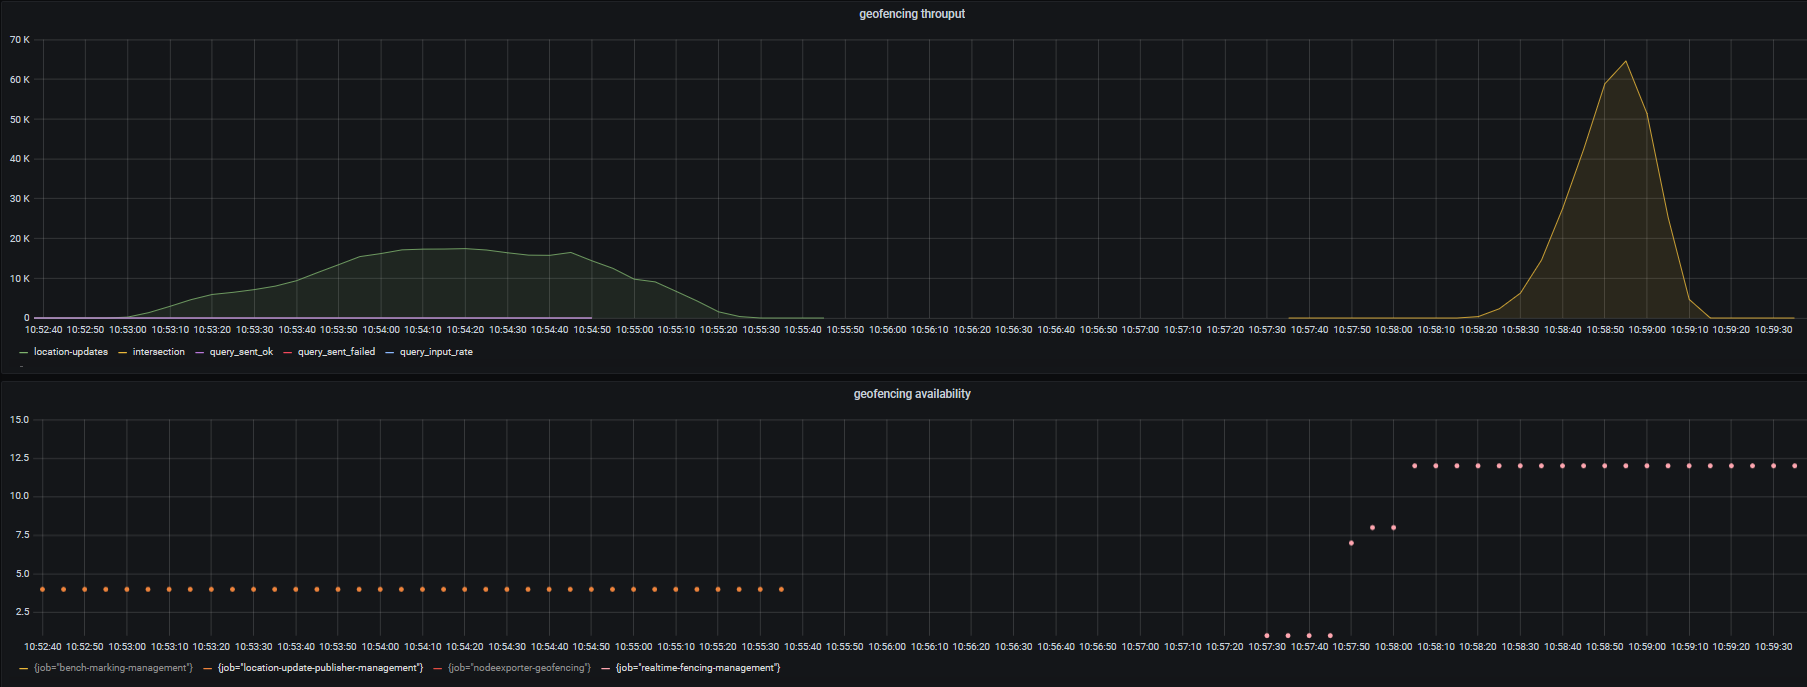
\includegraphics[width=\linewidth, scale=2]{images/evaluation/ex24-benchmarking-ongoing-1per2sec.png}
    \end{figure}

    In figure \ref{fig:ex24} the green line is input rate (number of location updates per second),
    yellow line represents throughput (number of fence point intersections) and the pink dots shows number of
    deployed instances of realtime-fencing.
    Orange dots illustrates number of up and running instances of location-update-publisher.
    We can clearly observe that after re-balancing among 10 newly deployed instance of realtime-fencing is finished,
    throughput has peaked very fast to about 65K fence-point intersections per second.

    \subsubsection{Conclusion of push leg free fall scalability evaluation}
    We can relay on buffering properties of stream processing systems for testing throughput of operators.
    Specially when producing input and process it on realtime involves too much IO latency.
    All in all, pull leg of FenceX has shown free fall scalability properties and ability to deliver throughput of
    ~65k/s.

    \clearpage


    \section{Related work}
    In this section we will go over a couple of papers which has introduced a geofencing systems and we compare them
    to FenceX.

    \subsection{Large Scale Indexing of Geofences}
    In \cite{Cirillo-Jacobs-Martin-Szczytowski-2014}, a poll style on demand geofencing system is introduced that supports large scales
    of data and load.
    This system has a concept of worker which refers to instances of application that answer to queries.
    As apposed to clients which send queries to the worker nodes.
    Dynamic caching and work load distribution over multiple instances of workers are the bases of achieved
    scalability.

    Each worker instance is responsible for indexing a region of the world, which allows for lower query and index latency.
    Since each worker instance is responsible for different part of the world, queries targeting border areas need
    special treatment.
    As a solution, each worker instance also is responsible for areas around its dedicated region.

    It is notable that software in \cite{Cirillo-Jacobs-Martin-Szczytowski-2014} uses a custom geospatial index,
    custom design and implementation.
    Using a custom index most probably means that the whole data is stored and processed in memory which allows for higher throughput.
    We will not, however, describe further the indexing strategy since it is outside context of this thesis.

    Throughput in \cite{Cirillo-Jacobs-Martin-Szczytowski-2014} is defined as number of location updates processed per second.
    Such processing involves updating an index plus a query to find a crossing geofence.

    When they are using benefit of localhost communication without any data replication involved (no availability), a
    throughput of 250k/s has been achieved on average.
    However, once they introduce data replication and inter server communication, the throughout drops to sub 10k/s
    range at best.

    \subsubsection{Comparison}
    The software introduced in \cite{Cirillo-Jacobs-Martin-Szczytowski-2014}, although having notification
    functionalities, is comparable to poll leg of FenceX.
    Both of them use load sharing (scale out) and in-memory data processing to achieve high throughput and
    scalability.

    FenceX, however, does not apply partitioning data among worker instances in poll leg, which makes it much easier to
    scale out.
    Also, the load balancing strategy when forwarding client queries to worker instances can be as simple as
    round-robin in FenceX.
    As a result, no throughput would be lost during load balancing.

    When it comes to numbers, FenceX has achieved a throughput in range of 15k/s compared to sub 10k/s for
    \cite{Cirillo-Jacobs-Martin-Szczytowski-2014}.
    Although \cite{Cirillo-Jacobs-Martin-Szczytowski-2014} has done wonderful when no availability was in action
    (no replication), we do not consider it a win over FenceX.
    FenceX has always been tested with full replication in action.
    So all in all, FenceX has achieved a higher throughout.

    \subsection{Using Complex Event Processing for implementing a geofencing service}
    A push style realtime geofencing system has been introduced in \cite{Nechifor_Comnac_2013}.
    It relies on a CEP (complex event processing) for fence entrance/exit detection.
    Which is comparable to functionalities of push leg of FenceX where realtime fence point intersections happen.
    System in \cite{Nechifor_Comnac_2013} is using a classic 3 tiers monolith architecture.
    Unit of concurrency in \cite{Nechifor_Comnac_2013} is not clear.
    So it is not clear what are the bounds for scalability of the introduced system.

    Throughput in this system is defined as number of location updates processed per second.
    Evaluations have shown that it can has achieved throughput of around 20k/s.

    \subsubsection{Comparison}
    Unlike FenceX, \cite{Nechifor_Comnac_2013} does not seem to have any considerations for
    scalability and availability.
    Also, when it comes to throughput, push leg of FenceX has achieved 65k/s which is much higher than 20k/s.


    \chapter{Conclusion}
    During this thesis we have combined microservices and stream processing concepts in order to design, implement
    and evaluate a highly scalable resilient geofencing system called FenceX.
    FenceX can handle high input rates and deliver high throughput with low latency.
    FenceX supports two types of geofencing, on demand and realtime.
    The on demand part is achieved by having a fully replicated co-located in-memory geo aware database.
    The realtime part is brought about using a distributed join over a partitioned table of fences and an ongoing
    stream of location reports.

    The result was so scalable that in most evaluation scenarios, we ran out of resources for producing more load
    before we can hit the upper bound of throughput (with a given deployment config).
    At best we have observed that FenceX can easily handle about 65K fence-point intersections and 15K queries (query by
    fence) per second.
    FenceX also has proven to have strong and weak scalability characteristics.

    When it comes to resiliency thanks to replication, scaling out (instead of up), re-balancing features of kafka
    consumers and highly decoupled components, FenceX has demonstrated being reliable under non-ideal conditions.


    \section{Future work}
    During our evaluations, we have used only one type of data collected from real taxi trip.
    Evaluating FenceX using data collected from people walking in an area can be also very insightful.

    Apart from the data, the implementation of our bench-marking application might have potential to be improved so
    that more load can be produced with less resources consumed.

    And in terms of features, pattern detection can be the next step for FenceX.
    Patterns that can be detected while observing events in windows of time.
    For example when a mover enters a no-go area and gets back out within seconds, an alarm might not needed to be
    generated.
    Currently, FenceX just detects enter/exit events on a one by one basis.



    \part[Stateful FAAS]{FenceX: Stateful Function as a serivce platform}


    \chapter{FenceX as FAAS provider}
    FenceX apart from being a geofencing system as described in the previous part of the report, can also be
    considered as an implementation for idea of function as a service.
    Stateful function as a service actually.
    In a sence, geofencing is just one special usage our system.
    So other types of computation can also be implemented in the same way without changing the architecture in any
    significant manner.
    In the following sections we will explain what is FAAS and how FenceX is a FAAS provider.


    \section{FAAS}
    Imagine a start up company is shaping around a brilliant brand-new audio compression algorithm.
    Two computer science engineers came up with an algorithm and now want to make money out of it.
    They don't want to publish any software or library but an online service, a few APIs (HTTP for example) only.
    They are confident enough in their work to know that once their service is up and running, a lot of companies
    want to use their service right away.
    Which means huge number of requests to handle.
    So however they design and implement a system around their algorithm, it should be highly scalable and efficient.

    Based on what we described about resilient highly scalable systems with high throughput, they should select
    microservices as architecture for their software behind their APIs.
    They need to sit and design different microservices, hire developers to help them with implementation and
    maintenance, hire an operations team for maintaining container orchestration tools (among others), and so many
    other activities before even they can start coding.
    Let alone deploying a feature into production

    However, they are thinking about a short time to market since they have noticed an opportunity soon to pop up in
    market for their service to be used vastly.
    Also, since they are a small startup, they are low on the budget.
    Most probably they can only hire one part-time front-end developer to create a website for introduction
    purposes.

    So far apparently they can not achieve a highly scalable system.
    What if they could just focus on the implementation of their algorithm?
    Just like they are implementing a function in the middle of nowhere.
    A C function, or a python function for that matter.
    They are implementing an audio compression algorithm.
    After all it's just some calculation and computation over an input then producing an output.
    So what if they could just implement that function, give it to a cloud service with promise of no more work
    required for exposing the API to internet.
    The compression algorithm will be exposed to internet as an HTTP API.
    It can also be configured to be triggered upon receiving a Kafka event, grpc call, AMQP message and much more .
    The start up people won't need to be worry about anything else.
    The cloud provider will take the code, build it somehow, and bring enough instances of the resulted artifact up and
    running according to the incoming load.
    So dynamic scalability out of the box.

    Payment will be based on number of processed requests or running time of functions.

    Any change to the code will be just changing a function.

    What we just described is the sell speech for the function as a service idea.
    Which is provided nowadays by most cloud providers.
    AWS lambda\cite{lambda} is the most famous one.


    \section{Stateless FAAS}
    In FAAS model, apart from separating business logic and execution platform, storage is also separated from
    execution platform.
    That is because of storage being not easy to scale in a distributed fashion.
    As a consequence, having very small computation units working totally decoupled, comes with price of not being
    able to access storage.
    Or not being able to access storage in the classic way.
    IO is usually an expensive operation regardless of execution model.
    When it comes to FAAS, IO becomes much harder to achieve due to following reasons:

    \paragraph{Network:} Since there is no storage and file system attached to each function, all IO should happen
    over network which brings about high latency which reduces throughput as a result.

    \paragraph{Run time limitation:} Each function, once called, has a limited time to live.
    If computation does not finish during the time limit, there will be no more chance to continue it.
    The high latency of IO over network does not match this limitation.

    \paragraph{Decoupled context:} Since all the running instances of the function are totally decoupled, there is
    no way for them to share something, a connection to database for example.
    So each time a function requires database or storage connection, a brand-new connection should be created.
    Which results in unnecessary latency, too many connections and loss of execution time budget.

    As a result, FAAS model is better to be used for stateless operations.
    Creating a thumbnail for an image, compressing an image or compressing a piece of audio.
    All the required computation can be carried out without need for storage or database.

    So what about stateful operations?
    Can't we enjoy the high level abstraction of FAAS model with stateful operations?


    \section{Stream processing and Stateful FAAS}
    For developers (users of FAAS platform), the function they implement has only some inputs parameters and an output.
    The input parameters can be driven from the triggering event/request/message.
    This is not different from implementing operations in a stream processing pipeline.
    Each stream processing operation, regardless of being stateful or stateless, is very similar to a function which
    has an input (triggering event) and an output (resulting event if any).
    For stateful operations, another input parameter exists which is the latest captured state for the key of the event.
    Please remember that in stream processing systems, events and states are key:value tuples.

    So we can actually implement a FAAS platform by modeling it as a stream processing pipeline.
    What we need is a source operation which has some adaptors.
    The adaptors turn an incoming request, HTTP for example, into a Kafka event so that operations down the pipeline
    can process them.
    Of course this implementation is asynchronous and eventually consistent.
    Paying that cost, brings about the benefit of stateful operations.
    Since we can just enjoy stateful operations in a stream processing pipeline in a highly scalable manner,
    a FAAS platform implemented by stream processing pipeline allows for definition of stateful functions as well.

    The only thing that users of system (developers) should do is to implement body of stream processing operations.


    \section{FenceX and FAAS}
    FenceX, as described previously, is a stream processing pipeline among many other things.
    It has both stateful and stateless operations.
    However, FenceX is designed in a way that operations are defined by architecture but their implementation should
    be provided as libraries.
    Each operation on execution, uses an object of a Java Class called Function.
    The mentioned library provides instances of those Functions.
    So such library can be provided by users of FenceX (developers) in the same way that FAAS users provide
    implementation for their functions.
    The signature of functions however is pre-defined due to architectural decisions.
    And the available operations to implement are also limited to what is needed for the architecture.

    So FenceX is an implementation for the idea of Stateful FAAS.
    It allows for distributed de-coupled highly scalable stateful function by limiting what function can be implemented.
    In a sense the implementation of those functions can be anything, so the limitation is more conceptual.

    Since FenceX needs that complied version of Functions, they can be implemented in pretty much any JVM language as
    far as they can be compiled into a Java class (Java byte code).
    Being language agnostic is another promise of FAAS idea which FenceX delivers to some extent.


    \section{Comparison}
    In this section we compare how FenceX has achieved stataful FAAS compared to another available work.

    \subsection{Cloudburst: stateful functions-as-a-service}
    In \cite{Functions-as-a-Service-2020}, to achieve stateful FAAS, co-location of cache and functions has been
    taken into action.
    Each function accesses the cache as storage of state.
    Functions are executed by function executors which are deployed in virtual machines.
    For each virtual machine, one cache instance exists.
    In order to keep the caches consistent, they are backed by an auto-scaling key:value store called Anna.
    And Anna uses lattice composition to fight inconsistency.

    Anna also, has a ACID2 conforming function called merge which is used by \cite{Functions-as-a-Service-2020} in
    order to gain high scalability.

    Table \ref{table:fencex-comp} compares FenceX with the solution provided by \cite{Functions-as-a-Service-2020}.

    \begin{table}[h!]
        \begin{tabular}{ |l|l|l| }
            \hline
            Property/System          & FenceX                    & \cite{Functions-as-a-Service-2020} \\
            \hline
            Consistency              & Eventual                  & Strong                             \\
            Statefulness strategy    & Stream processing         & Co-located caches                  \\
            ACID2 conforming         & yes                       & yes                                \\
            Data replication         & yes                       & yes                                \\
            Function execution retry & yes                       & yes                                \\
            State as KEY:VALUE data  & yes                       & yes                                \\
            Custom functions         & practically yes           & yes                                \\
            Underlying system        & Kafka/Spring/KafkaStreams & Anna                               \\
            \hline
        \end{tabular}
        \caption{Comparison of  \cite{Functions-as-a-Service-2020} with FenceX}
        \label{table:fencex-comp}
    \end{table}


    \section{Future work}
    FenceX is only the core/kernel part of a FAAS platform.
    In order to make it a fully functioning cloud service, some other tools and layers should be built around and
    upon it.
    For example, a web UI in which developers implement their functions (simple cases) and the system compiles
    the code itself and generate the library.

    Next step is to use that library to build microservices involved in FenceX.
    Then deploying them.
    This whole process can be automated.

    \nocite{*}
    \bibliography{sources}
    \bibliographystyle{IEEEtran}
\end{document}
